\documentclass[12pt]{report}

% General formatting
\usepackage[pdfusetitle]{hyperref}
\usepackage[a4paper, margin=1in]{geometry}
\usepackage{parskip}

% Include citations, and include bibliography in contents
\usepackage[nottoc]{tocbibind}
\usepackage{cite}

% Straight quote marks in code samples
\usepackage{textcomp}
\usepackage{upquote}

% Allow highlighting text
\usepackage{soul}

% Drawing and graphics tools
\usepackage{tikz}
\usepackage{dirtree}
\usepackage{graphicx}

% Allow landscape pages in document
\usepackage{pdflscape}

% Various operations on table cells
\usepackage{makecell}
\usepackage{multicol}
\usepackage{multirow}

% Allow inclusion of project proposal
\usepackage{standalone}


\usetikzlibrary{er}
\tikzstyle{plain} = [rectangle, rounded corners, text centered, draw=black]
\tikzstyle{trusted} = [rectangle, rounded corners, text centered, draw=black, fill=red!20]
\tikzstyle{untrusted} = [rectangle, rounded corners, text centered, draw=black, fill=yellow!20]
\tikzstyle{arrow} = [thick,->,>=stealth]

\title{Kerberos-based single sign-on with delegation for web applications}
\author{Daniel Carter}
\date {\today}

\begin{document}
\maketitle

\tableofcontents

\chapter{Introduction}

\section{Web Application Security}
\label{sec:web_application_security}
Many web applications are built around a database, which is used by the application framework to store user data and allow a user to view and edit it. In general, the user logs in using a username and password (which is checked by the web app framework itself), and the application then makes database queries on the user's behalf, processes the results, and displays them to the user in a suitable way.

In this scenario, the application framework has the ability to read and write arbitrary data in the database, and the only thing which prevents a malicious user from accessing data for which they have no authorisation to is the application code itself. This is potentially problematic, since web app authors are often not security experts and may accidentally cause data to be visible to the wrong users. Some examples of how this can occur include:

\subsection{SQL Injection}
\label{sec:sql_injection}
SQL injection is a form of command injection attack (which are currently number 1 in the OWASP \textit{Top 10 Web Application Security Risks} list\cite{OWASP10} and are therefore regarded as a significant problem in web app security). It occurs when an application uses a template database query such as
\begin{verbatim}
SELECT * FROM records WHERE username='$user';
\end{verbatim}
and replaces \verb+$user+ with a string that the user provides. However, with insufficient checking of parameters, a user can supply a string such as
\begin{verbatim}
' OR 1=1; --
\end{verbatim}
resulting in a total query of
\begin{verbatim}
SELECT * FROM records WHERE username='' OR 1=1; --';
\end{verbatim}
which returns the records of all users (since \verb+1=1+ is always true).

The following diagram represents an example of a typical current setup, and the problems that can be caused if an SQL injection vulnerability is present:

\begin{center}
  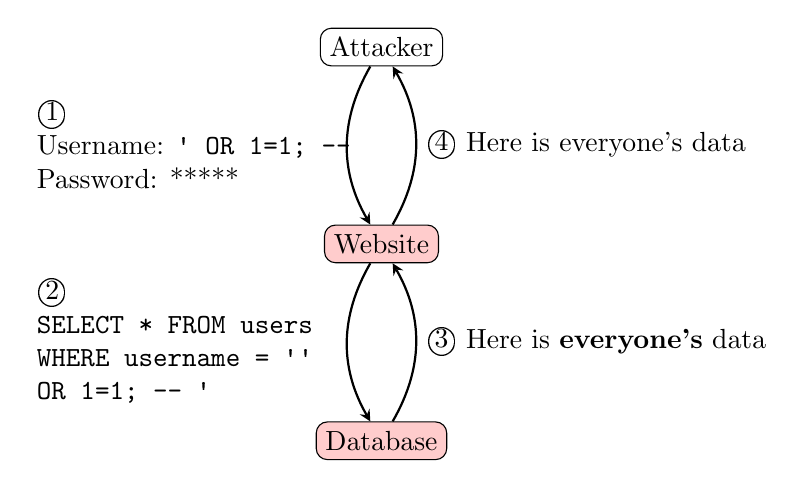
\begin{tikzpicture}[node distance=2.5cm]
    \node (user) [plain] {Attacker};
    \node (webserver) [trusted, below of=user] {Website};
    \node (database) [trusted, below of=webserver] {Database};

    \draw [arrow, bend right] (user) edge node {\parbox{0.65\textwidth}{\textcircled{1} \\ Username: \texttt{\textquotesingle \ OR 1=1; --} \\ Password: *****}} (webserver);

    \draw [arrow, bend right] (webserver) edge node {\parbox{0.65\textwidth}{\textcircled{2} \\ \texttt{SELECT * FROM users \\ WHERE username = \textquotesingle\textquotesingle \\ OR 1=1; -- \textquotesingle}}} (database);

    \draw [arrow, bend right] (database) edge node[right] {\textcircled{3} Here is \textbf{everyone's} data} (webserver);
    \draw [arrow, bend right] (webserver) edge node[right] {\textcircled{4} Here is everyone's data} (user);
  \end{tikzpicture}
\end{center}

In the diagram above, \textbf{red nodes} represent the Trusted Computing Base (TCB) of the system (i.e.\ the set of components which could cause the whole system to be compromised if that component contained a security vulnerability). In this setup, the website itself is a part of the TCB since a vulnerability in it could allow an attacker to take over the system.

In step 2, it is worth noting that the website can only steal data which is accessible to the user account used by the web app to log into the database. However, this is still likely to include the data of all users of the system since the web app needs legitimate access to user $A$'s data when $A$ logs into the system.

\subsection{Master Password Leakage}
There are many variations on master password leakage depending on exactly what was leaked, but these usually enable any malicious user to arbitrarily read and write from the database. Since the web app itself has these capabilities, it usually has a single username and password for authentication with the database, and these are usually stored in a simple configuration file. If the webserver is misconfigured such that the configuration file is visible over the internet, or if the file is accidentally checked into a public source control repository, an attacker can read this file, connect to the database server and read out all the data.

In a way, SQL injection is also a form of master password leakage even though the attacker does not actually see the master password; instead, they are able to abuse an application which holds a copy of that master password to perform malicious acts.

To demonstrate how significant a problem this is, a number of companies (such as GitGuardian\cite{GitGuardian}) have been set up simply to monitor online repositories for leaked security keys, and warn their owners. As a case in point, when setting up the test site for this project, the Django \texttt{settings.py} file initially contained a secret key that would allow an attacker to forge cryptographic signatures and so break the security of the application to an extent (but \textbf{not} gain full access to the database due to the application's structure, as detailed below). Although the key was moved to a file outside the repository (and changed, so that knowledge of the old secret key would be of no use to an attacker) before any files were made public, the mere existence of the secret key in a prior commit caused a warning email to be sent to me by GitGuardian within 70 minutes of changing the repository's visibility:

\begin{center}
  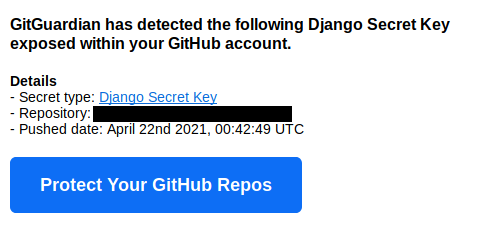
\includegraphics[scale=0.5]{01-gitguardian.png}
\end{center}

Even though this service only offers after-the-fact detection (a service which has genuinely leaked a secret key must quickly change this key everywhere it is used, and the site may still have been compromised in the meantime), the fact that businesses exist to perform these scans, and seemingly scan all public GitHub repositories to alert their owners, indicates the severity of this issue.

\subsection{Legal Implications}
As well as being commercially and reputationally damaging, unauthorised access to data can result in severe legal penalties: the Data Protection Act 2018 specifies a fine of up to 2\% of a company's global turnover (or 10 million Euros, if that is greater) may apply in cases of unauthorised disclosure of personal data\cite{GDPR}. Developing technologies that mean the web app does not have to be trusted with all data can significantly reduce the risk of these types of disclosure.

\section{Website Sign-on Systems}
A further disadvantage of having a ``local'' system of checking passwords on each website is that users are then expected to memorise a large number of different passwords, since otherwise a compromise of the password database of one website would allow the attacker to impersonate users on any other website where they had used the same password. Especially where several websites are ``connected'' in some way (e.g.\ by all being associated with the same organisation), a \textit{single sign-on} system can offer significant benefits.

A single sign-on (SSO) system generally consists of an authentication server, which collects a password (or some other security token) from the user and verifies the user's identity. When a user wishes to log on to a site that uses a particular SSO system, the user is redirected to the authentication server to log in. Assuming the login is successful, the user is redirected back to the site, along with some kind of unforgeable token to indicate that the authentication server has verified the user's identity.

Note that these steps only provide \textbf{authentication} of the user (i.e.\ that the person logging into the site is actually user $X$). \textbf{Authorisation} (i.e.\ checking whether user $X$ is entitled to access the site) must be done separately by the sites themselves.

The University's Raven authentication service is an example of an SSO system; numerous similar systems exist (including OAuth2, which also has the ability to do a form of ``delegation'' to allow one server to request resources from another, on behalf of the user\cite{Oracle-OAuth2}).

\section{Project Summary}
This project aims to produce an authentication system for web applications, such that a user can authenticate to a web application using a Kerberos ticket and the web application can use this ticket to obtain the user's data from a database.

Apart from the requirement that a user has a Kerberos ticket in the first place, this is set up to be completely transparent to the user -- the only action required is to visit the website and the authentication process will be carried out automatically (with the minor caveat that Kerberos authentication must be specifically enabled in most web browsers, although in a corporate environment this could be done centrally).

As a demonstration of this in practice, this project includes building an example file-browser application that performs all authentication and authorisation via Kerberos tickets and database permissions, rather than implementing the security in the web app.

While most of the library functionality to achieve this was already existent in some form, the actual completion of the project involved evaluating possible solutions and technologies for each part of the project, and adding functionality to libraries where this was required. The project also involved building the demonstration web application itself in order to provide a simple setup interface and demonstrate the correct working of the system.

Although involving the development of a web application and associated software patches, the main purpose of this project was to act as a feasibility study of using Kerberos-based authentication (and the associated ticket delegation) to websites. This is not a commonly used setup and many of the standards used with it (such as HTTP Negotiate) remain relatively little-known and obscure. Therefore, several areas of this project included research into different possible approaches for development before selection of a suitable technology, and in two cases patches to existing open-source projects were developed to add functionality not previously offered.

\section{Related Work}
The core Kerberos system and its extensions are described in a series of IETF RFCs, several of which are relevant to this project:

\begin{itemize}
\item
  RFC 2478\cite{RFC2478} describes the \textit{Simple and Protected GSS-API Negotiation Mechanism} (SPNEGO) which gives a (relatively generic) overview of negotiation-based authentication, where a server can provide information on what authentication methods it supports and the client can authenticate using one of these methods. This RFC illustrates examples of how the authentication process works, but is not tied to a particular protocol, and so is an important description of many of the overall concepts referred to in this project.
\item
  RFC 2743\cite{RFC2743} (along with several earlier RFCs) defines the current version of the Generic Security Service API (GSS-API) conceptually, using an exchange of tokens to prove identity and incorporating the concept of security tokens being delegable to another system or process. Principles stated here include that of the tokens being ``opaque from the viewpoint of GSS-API callers'', where the user of a system simply requests a ticket and then passes it to the appropriate service without the user attempting to extract the contents of the ticket. RFC 2744\cite{RFC2744} lays out a concrete API for RFC 2743 in the form of C language bindings.
\item
  RFC 4178\cite{RFC4178} describes, at a conceptual level, a negotiation framework for GSS-API systems to select an authentication system which they are both compatible with. Under this setup, the system initiating a connection offers a set of mechanisms which it can use to connect, with an order of preference. The system being connected to can then use the highest-preference system which it is capable of using, or refuse the connection if none of the suggested mechanisms is suitable.
\item
  A later RFC (RFC 4559\cite{RFC4559}) refers to a Windows-based system which allowed a user to log into a web application, from which a suitably equipped application could delegate the ticket to another system such as a database server. This was included by Microsoft in IIS 5.0 by virtue of adding a ``Negotiate'' extension to the HTTP protocol for use with Kerberos, and permitted a user to log in to the website without needing a password as described above in the aims for this project.
\end{itemize}

The ``HTTP Negotiate'' extension was subsequently included in various open-source web browsers. It also has some support in the Apache web server, and the aim of this project is effectively to replicate Microsoft's setup of a Kerberos-based single sign-on with delegation using an open-source web framework (Django), in conjunction with the Apache web server and any client web browser which supports the Negotiate extension.

\chapter{Preparation}

\section{Kerberos}
The Kerberos protocol works based on a system of \textit{tickets}, which are managed by a \textit{Key Distribution Centre} (KDC). The basic requirement of the system is to allow a centralised database of users (for example, the main user database in an office) who can demonstrate their identity in order to log in to applications and services, but \textbf{without} having to store or transmit passwords or other long-term secrets on potentially untrusted machines.

A very commonly used implementation of the Kerberos protocol is found in Microsoft's Active Directory system, which is used by many organisations to centrally co-ordinate logins and access to resources on Windows PCs on a corporate network. With only slight modifications, the setup illustrated in this report could be used with a pre-existing Active Directory server to provide a single sign-on system for an organisational intranet or similar.

In both Microsoft-based and open-source implementations, LDAP (Lightweight Directory Access Protocol) databases are commonly used to hold user information. At the most basic level, these hold a set of users and corresponding \textit{attributes} (which could include information about how the user is allowed to log in, which resources that user is allowed to access and so on). The LDAP database also holds information about non-human \textit{principals} (which could be systems such as web or database servers) and so, as explored in \autoref{sec:kerberos_ticket_delegation}, can be used to set delegation permissions from one system to another.

The basic workings of the Kerberos protocol are as follows:

\begin{itemize}
\item
  A user initiates a session by requesting a Kerberos ticket from the KDC, authenticating with a password.
\item
  The KDC returns a \textit{ticket-granting ticket} (TGT), and returns it encrypted using the user's password.
\item
  The user decrypts the TGT, and the user's machine can then discard the stored password.
\item
  When the user wants to access a service, the user sends the TGT back to the KDC along with an identifier for the service to be logged into.
\item
  The TGT grants the user a \textit{service ticket}, which the user then passes on to the service. The service is then able to use that ticket for authentication.
\end{itemize}

The following listing shows a client which has obtained both a TGT and a service ticket. The ticket in the first line (\verb+krbtgt/LOCAL@LOCAL+) is the \textit{ticket-granting ticket} which the client obtained when first authenticating to the KDC, and the second line contains a \textit{service ticket} (\verb+HTTP/krbsite.local@LOCAL+) to log in to the \verb+HTTP+ service on \verb+krbsite.local+ (i.e.\ to access the web page hosted on that server).

\begin{quote}
\begin{verbatim}
$ klist
Ticket cache: FILE:/tmp/krb5cc_1000
Default principal: user1@LOCAL

Valid starting     Expires            Service principal
05/05/21 14:54:18  06/05/21 00:54:18  krbtgt/LOCAL@LOCAL
	renew until 06/05/21 14:54:18
05/05/21 14:54:25  06/05/21 00:54:18  HTTP/krbsite.local@LOCAL
	renew until 06/05/21 14:54:18
\end{verbatim}
\end{quote}

As shown in the command output above, Kerberos tickets have an initial expiry time and a ``renew until'' time. The latter allows a user to remain connected to a Kerberos system for longer without having to re-authenticate, but reduces the potential risk of an unattended ticket being usable later since a ticket cannot be renewed after it has expired.

\section{SPNEGO}
SPNEGO (Simple and Protected GSSAPI Negotiation Mechanism) is a mechanism which uses a single packet exchange to identify a suitable protocol to authenticate the user with. In practice, it is usually used with either NTLM (a different challenge-response protocol) or Kerberos. NTLM is non-ideal in practice because it involves using the hash of a user's password as a long-term key, meaning that a key that is stolen from a compromised machine can continue to be used until the user's password is changed (whereas stolen Kerberos tickets are not practically useful since they expire within a relatively short period of time).

The server can specify which protocols it is willing to accept. For example, using the \verb+mod_auth_gssapi+ Apache module used here, the following directive ensures that only Kerberos (\texttt{krb5}) authentication will be accepted for GSSAPI:

\begin{verbatim}
GssapiAllowedMech krb5
\end{verbatim}

A full copy of the \verb+.htaccess+ file which configures many options in Apache for this project, is included in \autoref{sec:appendix1}.

\section{Kerberos Backend}
\label{sec:kerberos_backend}
The KDC and related Kerberos backend services are a significant component of the system, and form part of the \textit{trusted computing base} of the setup (see \autoref{sec:sql_injection}). Although not actually requiring any new software development (since in a real situation this backend would already exist, for instance as an Active Directory server), arranging a suitable test setup with the right permissions was required for the project.

\subsection{Basic MIT Kerberos Backend}
The default backend used by MIT Kerberos is based on Berkeley DB and simply creates a set of 4 files in which to store information on the principals using the system\cite{KDC-database-docs}. While simple to set up (and what I used initially when experimenting with running a Kerberos server), the basic backend does not have sufficient functionality to support constrained delegation of tickets to another system as it is missing the required access control functionality\cite{KRB-DELEG}. Because this was a goal of this project, the Berkeley DB-based system was not suitable.

\subsection{Connecting to an LDAP Server}
Using the \texttt{kldap} module, a suitably configured LDAP database can be used as a data store for Kerberos principals. This offers additional flexibility above what is possible using the basic backend, and (crucially) allows attributes to be set to define what permissions a given principal has for delegation. This is explored further in \autoref{sec:kerberos_ticket_delegation}.

\section{Kerberos Ticket Delegation}
\label{sec:kerberos_ticket_delegation}
In addition to use for authentication, Kerberos supports a method of \textit{delegating} tickets. This means that a principal $A$ can pass a ticket to a service $X$ as a means of authentication, and $X$ can pass the ticket on to a third system $Y$ to request resources on the user's behalf.

This is valuable because it means that $X$ can access resources which ``belong'' to $A$, without $X$ needing to have direct access to $Y$. This means that less trust in $X$ is needed (since it does not need privileged access to $Y$), and so the types of attacks discussed above become much less likely.

\subsection{Methods of Delegation}
Kerberos supports several methods of delegation, and I investigated these when researching the best method to set up the web application. Broadly, there are three ways of controlling what data is accessible to an application $X$ at a given time: which users' tickets the application actually has, how long those tickets last before expiring, and on which other servers $X$ is able to use those tickets.

\subsection{Unconstrained Delegation}
The traditional, and simplest, method for delegation is simply for the user $A$ to pass their ticket-granting ticket to the service $X$. $X$ can now behave as though it were $A$, and access any resources to which $A$ has access by simply presenting $A$'s ticket-granting ticket to the KDC and requesting a suitable service ticket\cite{JohnKol-unconstrained-deleg}.

In MIT Kerberos, this is achieved by marking service $X$ with the \verb+ok-as-delegate+ flag, which ``hints the client that credentials can and should be delegated when authenticating to the service''\cite{KDC-conf-docs}.

Despite seemingly being no better than $A$ simply giving a password to $X$ (so that $X$ can log in ``as'' $A$ when accessing $Y$), this scheme offers some advantages:

\begin{itemize}
\item
  Kerberos tickets are time-limited, so if $A$ no longer wishes to allow $X$ to access resources, all $A$ has to do is wait for any delegated tickets which $X$ currently holds to expire (and not send any more, although if $A$ sent a ticket that was renewable it may be necessary to wait for the ``renew until'' time has passed to be sure that it cannot be used). This contrasts with passwords which are valid until the user changes them, may well not be straightforward to change in a complex corporate network and could have been re-used by users on other systems.
\item
  Some limitations are placed on what can be done with the tickets. Although $X$ can use the TGT to get a service ticket to any other system $Y$ that $A$ can access, $Y$ does not automatically have the right to delegate this ticket further. If $Y$ does \textbf{not} have the \verb+ok-as-delegate+ flag set, then $X$ can \textit{access} $Y$ on $A$'s behalf but not allow $Y$ to perform actions for $A$ on some other server $Z$. If $Y$ is not well-trusted, this can be a significant benefit. Additionally, tickets sent in this way can be bound to IP addresses, to limit the risk that they are passed on to insecure other systems.
\end{itemize}

While the second of these advantages is significant, it may still not offer enough access control over the network. In particular, $A$ cannot give $X$ the ability to delegate to $Y$ without also giving $X$ the ability to delegate to \textbf{any} other service which $A$ has access to. In many cases this would be too great a risk; it may well be desirable to allow $X$ to fetch $A$'s work documents from $Y$ to display them in a web app, but not to allow $X$ to retrieve $A$'s financial records from another system $Z$ within the same Kerberos realm.

In this case, constrained delegation offers a far more controllable method of only allowing services to delegate tickets in particular ways, at the expense of a more complex setup for managing applications.

\subsection{Constrained Delegation (S4U2proxy)}
The \textit{Service for User to Proxy} (S4U2proxy) system is a Microsoft-designed extension to the basic Kerberos setup that allows one service $X$ to obtain a service ticket to another service $Y$ (on behalf of a principal $A$) in a controlled manner. Once service $X$ has been marked as ``permitted'' to obtain tickets for service $Y$, it can do so simply by making a request to the KDC, without having any need to know the user's Kerberos password\cite{MS-s4u2}.

Unlike with unconstrained delegation, here the ticket-granting ticket is not passed over to $X$; instead, $X$ is given a service ticket from $A$ as normal (to prove $A$'s identity and that $A$ wishes to connect to $X$). When $X$ needs to access $Y$ on behalf of $A$, $X$ \textit{submits the service ticket} to the KDC. If the permissions in the KDC are set appropriately, it is able to give $X$ a ticket to $Y$ on behalf of $A$.

This requires a more complex setup of permission models in the KDC than simply a list of principals, since the KDC must now decide which services can delegate tickets to which others. As discussed in \autoref{sec:kerberos_backend}, an LDAB backend allows the relevant \texttt{krbAllowedToDelegateTo} permission to be set on the user\cite{KRB-DELEG}.

In addition to the advantages described above for unconstrained delegation, there are some further advantages here:

\begin{itemize}
\item
  Much richer customisation of access control is possible. The system can now be set up so that $A$ can log into $X$ and have a Kerberos ticket delegated to $Y$, or log into $P$ and have a ticket delegated to $Q$, but not allow $X$ to delegate to $Q$. There is no simple set of ``privileged'' applications which are allowed to perform (all) delegation, but a customisable set of permissions between systems, and so applications which simply need to request some data from another server can be assigned restrictive access permissions and do not need to be part of the trusted computing base.
\item
  The number of powerful ticket-granting tickets that are stored in systems on the network is reduced. If an attacker gains access to $X$, the attacker will, at most, get service tickets for all users who have recently logged into $X$ (i.e.\ who have logged in and whose stored tickets have not yet expired), and delegated service tickets to the services which $X$ is allowed to. The attacker does not get a ticket-granting ticket to use on arbitrary applications.
\end{itemize}

In this project, the permitted delegation patterns are described using records in the LDAP database. The following pattern is therefore used on the LDAP server to set the \texttt{krbAllowedToDelegateTo} attribute on \verb+HTTP/krbsite.local+ to \verb+postgres/krb.local+ (which allows delegation from the web server on \verb+krbsite.local+ to PostgreSQL running on \verb+krb.local+):

\begin{verbatim}
dn: krbPrincipalName=HTTP/krbsite.local@LOCAL,cn=LOCAL
,cn=krbContainer,dc=local
changetype: modify
add: krbAllowedToDelegateTo
krbAllowedToDelegateTo: postgres/krb.local@LOCAL
\end{verbatim}

Under Microsoft Active directory, a similar setting named \texttt{msDS-AllowedToDelegateTo} is available, and this can be used in effectively the same way as above to enable constrained delegation from one service to another\cite{MS-deleg-attribute}.

\subsection{S4U2self}
This description is included here for completeness (because of its similar name) although it is \textbf{not} a true method of delegating tickets.

The Microsoft standard document for S4U2self\cite{MS-s4u2} states that:

\begin{quote}
  The S4U2self extension allows a service to obtain a service ticket to itself on behalf of a user. The user is identified to the KDC using the user's name and realm. Alternatively, the user might be identified based on the user's certificate.
\end{quote}

In effect, Kerberos authentication is bypassed completely and the server $X$ is able to get a ticket for $A$ simply by specifying $A$'s user name. This may be useful in some situations if not all clients can use Kerberos, but it offers a significantly weaker security model (since $X$ can now obtain service tickets for any user) and so if $X$ is compromised then records from all users can be gathered. As the aim of this project is to reduce the amount of trust placed in applications such as $X$, S4U2self is not relevant to this goal and will not be considered further.

The ability of $X$ to get a delegable ticket using S4U2self can be controlled in the KDC, and so (for example) the following command is used to stop the web server from being able to to so:

\begin{verbatim}
modprinc -ok_to_auth_as_delegate HTTP/krbsite.local@LOCAL
\end{verbatim}

\section{Storage of Credential Caches}
\label{sec:storage_of_credential_caches}
Ignoring two Windows-specific mechanisms, MIT Kerberos offers five methods of storing credential caches\cite{MIT-ccache-types}:

\begin{itemize}
\item
  \textbf{FILE} mode stores the credential cache into a file on the server's filesystem. This offers the best built-in support in existing modules, but its default configuration is vulnerable to having tickets stolen if the webserver is compromised (see below).
\item
  \textbf{DIR} (directory) mode places all tickets in the supplied credential cache into a particular directory. In this case (since $A$ only needs to supply one ticket to $X$) this has no advantage over \textbf{FILE}.
\item
  \textbf{KEYRING} mode uses a feature of the Linux kernel to store credentials in an area of private memory. This has the advantage over many of the methods listed here that a kernel keyring can be made process- or thread-specific and so prevent other threads gaining access to private credential caches.

\item
  \textbf{MEMORY} caches are conceptually similar to keyring-based caches except they are not Linux-specific and offer less granularity in setting access permissions. Many of the same issues described above also apply to this cache type, particularly in relation to removing access from threads.
\item
  \textbf{KCM} mode was recently added to MIT Kerberos, and uses a specific daemon process to manage credential caches. Although potentially offering advantages over simpler systems (and being less OS-specific than \textbf{KEYRING}), it is still primarily tied to the UID of an operating system user account and so does not offer much security between different tickets held by the same server user. Since having a separate login account on the web server for each database user would normally be impractical, this limits the usefulness of this option.
\end{itemize}

\section{SQL Access Control}
\label{sec:sql_access_control}
A core aspect of this project is the ability to shift access control from the web app itself to the SQL server. Most SQL server applications contain permissions models which allow selective access to data, and there are often a number of ways of achieving this (especially since they are not very well standardised across SQL implementations). As this project specifically uses PostgreSQL, I evaluated several methods to determine how best to implement the security protocol.

\subsection{Basic SQL Permissions}
In many cases, the basic SQL syntax to allow or deny users access to a whole table may be sufficient. For example, if there is a table of ``sensitive'' information that only a certain group of employees are allowed to see, using simple SQL \texttt{GRANT} statements allows this to be set up without any further complexities. It is only in the case that users need access to specific rows within a table that more complex access control methods need considering.

\subsection{\texttt{SECURITY DEFINER} Functions}
As with most SQL implementations, PostgreSQL allows the definition of stored procedures using the \texttt{CREATE FUNCTION} operation. This allows a pre-written operation, which performs a series of actions and may make changes to the database and/or return a result, to be provided to users of the database.

Basic stored procedures do not have any specific security implications; they are merely a way of avoiding repeatedly executing the same code (and potentially offering performance improvements). However, PostgreSQL defines an additional construct that permits security management: the \texttt{SECURITY DEFINER} property.

A PostgreSQL function with this property specified runs ``as'' the user creating the function, regardless of who executes it\cite{postgres-SEC_DEF} (in a similar way to how the \texttt{setuid} bit works in Unix). This allows the database owner to create a function which can read the whole table and when run, perform some check based on the user calling it and return appropriate results.

These are effectively similar to Trusted Procedures in a Clark-Wilson security model, where data can only be modified by particular procedures which enforce constraints on the data. This therefore allows something of a separation of authentication (logging into the database, via Kerberos) and authorisation (where the procedures describe what access is permitted).

\subsection{SQL Views}
These effectively allow a new table to be created out of a view over an existing table. Using syntax such as the following, it is therefore possible to construct a new table which only has the calling user's data visible; the user can then be granted access to this view (which automatically selects data based on the user's own username) and does not then need to have any access to the original table. For web application purposes, it can be queried just like any other table.

\begin{verbatim}
CREATE VIEW my_files AS
SELECT f.*
FROM files_file f, files_permission p
WHERE f.id = p.file_id
AND p.owner = user;
\end{verbatim}

Write access cannot be directly granted in this way for views containing cross-table joins, but can be achieved either by using \texttt{ON INSERT} rules in the same way as the \texttt{ON SELECT} rules below, or by using SQL triggers\cite{postgres-CREATE_VIEW}.

\subsection{Use of \texttt{ON SELECT} to Redefine Selection}
PostgreSQL also allows rules to be created which effectively redefine actions on tables. For example, a rule could be used to replace the default \texttt{SELECT} rule on the table storing file information with one that checked user permissions.

However, this is likely to introduce unnecessary complexity (particularly with ensuring that administrators can still access data as necessary, for example). For these reasons, the PostgreSQL documentation considers it ``better style to write a \texttt{CREATE VIEW} command than to create a real table and define an \texttt{ON SELECT} rule for it''\cite{postgres-CREATE_RULE}.

\subsection{Row-level Security}
The final method considered, and the one which turned out to be best-suited to this problem, was PostgreSQL's row-level security constructions. These allow policies (defined by the database owner) to determine who can view or modify which rows in the database, and is well-suited to tasks like this.

See \autoref{sec:implementing_database_access_control} for more information about how these were actually used.

\section{Requirements Analysis}
There are three broad components to the setup of this project: the web server, the web application framework and the database.

Of the available open-source web server frameworks, Apache and nginx are two which receive significant use. Both have some form of existing Kerberos support and so this project could probably have been completed using either. As Apache is the only one of the two with which I had any previous experience, I decided to continue using it following some experimentation over the summer (see ``starting point'' below). Apache's module system is also more flexible than nginx's, which offers advantages in this project.

For the web application framework there are many more options, from a basic setup with PHP files to more full-featured systems. Although there would likely have been many good candidates, I selected Django as a widely-used framework which offers the required features (and is written in Python, which is a language that I was previously familiar with).

Finally, there are also a number of possible options for the SQL server running the database. Although my previous SQL experience was primarily using mySQL, PostgreSQL offers more advanced functionality in a number of areas (including flexibility in table security options) and so offers advantages for this project. It also offers built-in support for authenticating to the database using a Kerberos ticket, which is clearly of use here.

\subsection{Source Code Management}
For the Django directory itself, running it as a git repository with commits pushed to GitHub provides both version control and a backup of the directory in use. This was also checked out into a separate folder on my PC which was backed up to Dropbox, to provide an additional layer of backup.

Since the main development was completed in virtual machines which would have been time-consuming to set up again if lost, I also took backups of the whole VM setup to an external hard drive during development. In the event of a failure, I could have restored these backups to a replacement PC to continue working on them.

\subsection{Testing Methodology}
Since the core aims of the project are to provide a secure system, this can be most appropriately tested using a security analysis of the types of vulnerabilities (such as SQL injection) which it is vulnerable to, and how this compares with other systems in current use. As a na\"ive implementation of the project also has the potential to result in slower performance than existing systems (due to extra authentication overheads), evaluation of performance and comparing it with a non-Kerberos based system is also a component of evaluating the system.

\section{Starting Point}
(N.B.\ the text below is a slightly modified version of the starting point submitted in my project proposal)

Kerberos support for Apache already exists (via the \verb+mod_auth_gssapi+ module), and this includes some ability to delegate tickets although with drawbacks (principally that the tickets to be delegated are placed in a directory which is accessible to any process running as the webserver user). Django similarly includes Kerberos extensions (such as \verb+django-gssapi+), but these do not directly offer any delegation facilities and are ultimately not really relevant to this project since Django does not need to participate in Kerberos authentication other than passing on login information. As a starting point, I have investigated these and built on the functionality which they already offer.

PostgreSQL already has support for Kerberos and this can be used as a back-end database system.

I previously had some knowledge of authentication systems and general security topics from the 1B Security course, and of C programming from the 1B Programming in C and C++ course (although Apache includes several specific libraries that differ from those used in ``normal'' C programming\cite{Apache-book}). I have also had general experience with web application setup (although not the specific technologies involved here, which required learning how Django works and the syntax of its templating language) through the 1B Group Project and work done outside the Tripos.

In addition, over the summer vacation I did some experimentation with Kerberos authentication to set up a virtual machine using the existing Kerberos functionality of Apache and PostgreSQL (logging in separately to the two applications without any delegation of tickets).

The Django documentation\cite{Django-docs} was used as a reference and guide throughout development, including using (some of) the provided tutorial to set up the basic web app before being integrated with the Kerberos authentication setup.


\chapter{Implementation}

\section{Project Structure}

\subsection{Overall Structure}
The overall structure of the authentication process is as shown below.

\begin{center}
  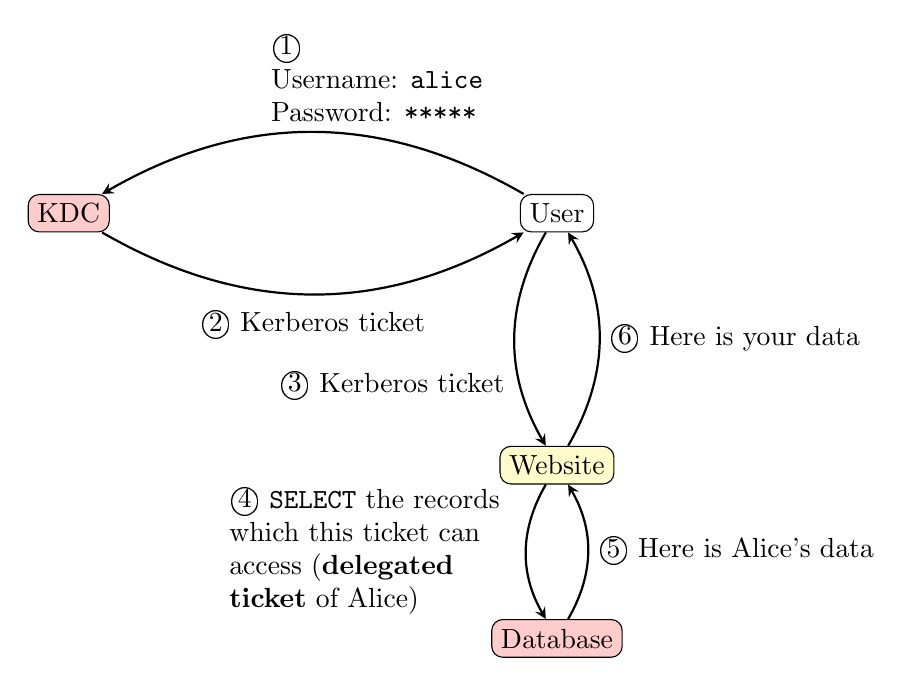
\begin{tikzpicture}[node distance=2.2cm]
    \node (user) [plain] {User};
    \node (webserver) [untrusted, below of=user, yshift=-1cm] {Website};
    \node (database) [trusted, below of=webserver] {Database};
    \node (kdc) [trusted, left of=user, xshift=-4cm] {KDC};

    \draw [arrow, bend right] (user) edge node[above, xshift=2.5cm] {\parbox{0.5\textwidth}{\textcircled{1} \\ Username: \texttt{alice} \\ Password: \texttt{*****}}} (kdc);

    \draw [arrow, bend right] (kdc) edge node[above, yshift=-0.7cm] {\textcircled{2} Kerberos ticket} (user);

    \draw [arrow, bend right] (user) edge node[left, yshift=-0.6cm] {\textcircled{3} Kerberos ticket} (webserver);

    \draw [arrow, bend right] (webserver) edge node[left] {\parbox{0.3\textwidth}{\raggedright \textcircled{4} \texttt{SELECT} the records which this ticket can access (\textbf{delegated ticket} of Alice)}} (database);

    \draw [arrow, bend right] (database) edge node[right] {\textcircled{5} Here is Alice's data} (webserver);
    \draw [arrow, bend right] (webserver) edge node[right] {\textcircled{6} Here is your data} (user);
  \end{tikzpicture}
\end{center}

Since the same KDC can be used for many websites where the users all have a login to the same Kerberos realm, the system also functions as a single sign-on system (using the Kerberos ticket as proof of identity). As described in \autoref{sec:kerberos_ticket_delegation}, this means that none of the individual websites need to be given access to the user's password, they are not able to arbitrarily impersonate the user on other systems, and they cannot get any data from other systems which they have not been authorised to access. A website also cannot get data on behalf of users for whom it does not hold a live Kerberos ticket (so there is no way to access the records of users who have not used the system for a time interval at least as long as the expiry time of their tickets).

Note that, unlike in the diagram shown in \autoref{sec:sql_injection}, the web application no longer has to be part of the trusted computing base; it merely passes on the Kerberos ticket which a user has provided and does not have any other method of accessing the data in the database. This means that an attack such as the one depicted in \autoref{sec:sql_injection} cannot take place.

\subsection{Demonstration Web Application}
The project demonstrates a web application that uses Kerberos authentication and delegation to fetch data from a database and display it to the user, in the form of a basic file browser-type application. Django makes use of a structure based on \textit{models} which correspond roughly to classes in the object-oriented programming model (and are represented by Python classes in the Django configuration), with each model being able to have different attributes (which are set up as member variables of the class). When stored in a database, each model is a table, with each object of a model being a row in that table and each attribute being a column.

In the example web app, the models are files and directories, plus associated tables to hold access permissions for both files and directories. The database model can be represented in the following entity-relationship diagram:

\begin{center}
  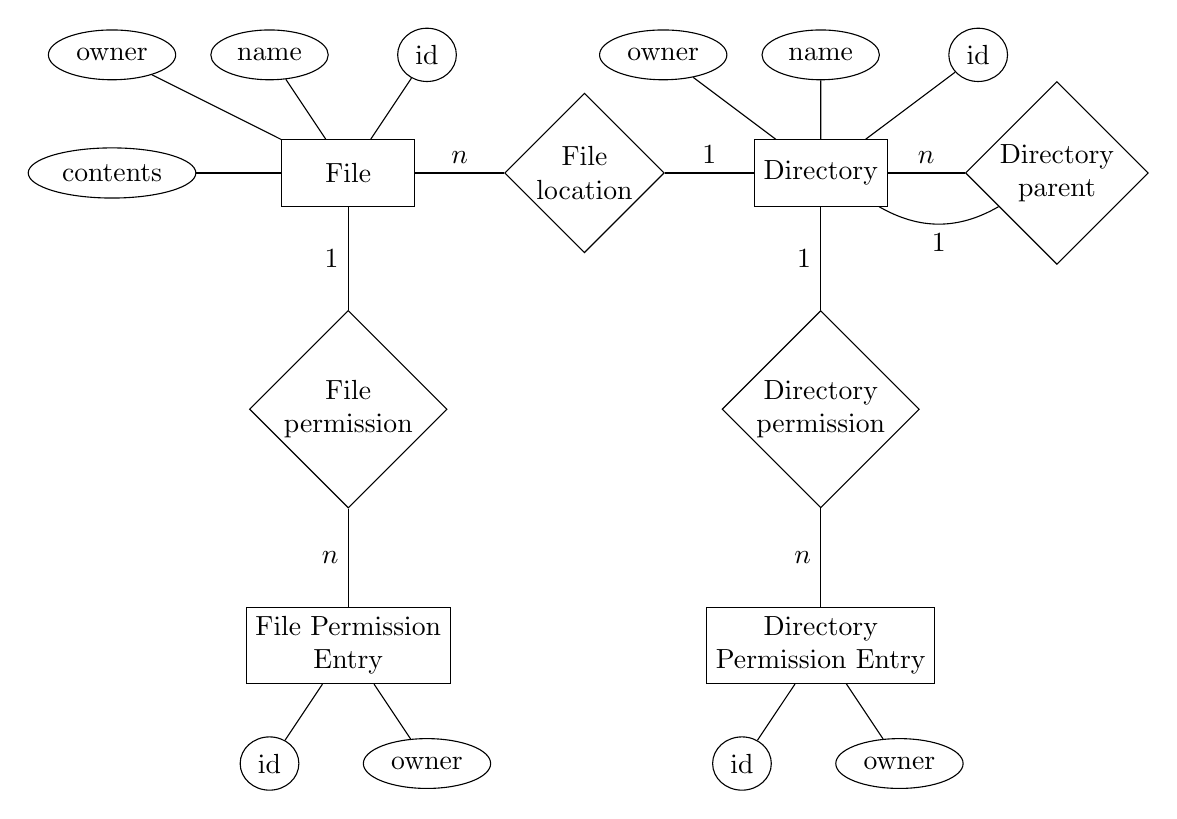
\begin{tikzpicture}[node distance=3cm]
    \node[entity] (file) {File}
         [grow=up, sibling distance=2cm]
         child {node[attribute, left of=file] {contents}}
         child {node[attribute] {id}}
         child {node[attribute] {name}}
         child {node[attribute] {owner}};

         \node[relationship, right of=file, align=center] (file_location) {File \\ location};

         \node[entity, right of=file_location] (directory) {Directory}
              [grow=up, sibling distance=2cm]
              child {node[attribute] {id}}
              child {node[attribute] {name}}
              child {node[attribute] {owner}};

              \node[relationship, right of=directory, align=center] (directory_parent) {Directory \\ parent};

              \node[relationship, below of=file, align=center] (file_permission) {File \\ permission};

              \node[entity, below of=file_permission, align=center] (file_permission_entry) {File Permission \\ Entry}
                   [sibling distance=2cm]
                   child {node[attribute] {id}}
                   child {node[attribute] {owner}};

                   \node[relationship, below of=directory, align=center] (directory_permission) {Directory \\ permission};

                   \node[entity, below of=directory_permission, align=center] (directory_permission_entry) {Directory \\ Permission Entry}
                        [sibling distance=2cm]
                        child {node[attribute] {id}}
                        child {node[attribute] {owner}};

                        \path (file) edge node [above] {$n$} (file_location);
                        \path (file_location) edge node [above] {1} (directory);

                        \path (directory) edge node [above] {$n$} (directory_parent);
                        \path (directory_parent) edge[bend left] node [below] {1} (directory);

                        \path (file) edge node [left] {1} (file_permission);
                        \path (file_permission) edge node [left] {$n$} (file_permission_entry);

                        \path (directory) edge node [left] {1} (directory_permission);
                        \path (directory_permission) edge node [left] {$n$} (directory_permission_entry);
  \end{tikzpicture}
\end{center}

\subsection{Database Setup Application}
The project also includes a component which performs the necessary setup tasks (setting up SQL permissions), so that all that is required for the user of the application is to:
\begin{itemize}
\item
  Set up a Django app with the appropriate models
\item
  Run the normal Django \texttt{migrate} command to set up the database
\item
  Use the web interface (created as part of this project) to set up appropriate access controls
\end{itemize}

\section{Repository Overview}
The core of this project is a Django web app, which is able to both perform the necessary setup steps to get the system working and (as a separate component) demonstrate the working of the system.

The structure of the directories involved is as shown below. The basic directory layout is as produced by the Django project setup procedure, with some files having ``stubs'' automatically generated by this process (as well as a default \texttt{settings.py} and the short \texttt{manage.py} script which is provided to run various application management steps).

\begin{multicols}{2}
  \dirtree{%
    .1 django-code.
    .2 files.
    .3 admin.py.
    .3 apps.py.
    .3 \hl{forms.py}.
    .3 \_\_init\_\_.py.
    .3 migrations.
    .4 \_\_init\_\_.py.
    .3 \hl{models.py}.
    .3 templates.
    .4 files.
    .5 \hl{create.html}.
    .5 \hl{dirview.html}.
    .5 \hl{fileedit.html}.
    .5 \hl{fileview.html}.
    .5 \hl{index.html}.
    .5 \hl{listing.html}.
    .5 \hl{permissions.html}.
    .5 \hl{rootdir.html}.
    .5 \hl{search.html}.
    .3 tests.py.
    .3 urls.py.
    .3 \hl{utils.py}.
    .3 \hl{views.py}.
    .2 (Continued in next column).
  }
  \columnbreak
  \dirtree{%
    .1 .
    .2 krbsite.
    .3 asgi.py.
    .3 \hl{filedb\_router.py}.
    .3 \_\_init\_\_.py.
    .3 \hl{middleware.py}.
    .3 settings.py.
    .3 urls.py.
    .3 wsgi.py.
    .2 managedb.
    .3 admin.py.
    .3 apps.py.
    .3 \hl{forms.py}.
    .3 \_\_init\_\_.py.
    .3 models.py.
    .3 templates.
    .4 managedb.
    .5 index.html.
    .5 \hl{result.html}.
    .5 \hl{table\_mapping.html}.
    .3 tests.py.
    .3 urls.py.
    .3 \hl{views.py}.
    .2 manage.py.
  }
\end{multicols}

The top-level directories represent the separation of ``components'' in the Django setup, with \texttt{krbsite} containing whole-system configuration, \texttt{files} containing the setup of the demonstration file manager application, and \texttt{managedb} having the code for the database setup application.

The primary code files are those highlighted above, with the most substantial code additions being in the \texttt{views.py} files for both \texttt{files} and \texttt{managedb} (since these contain the main logic for constructing web pages in the file browser and database management apps respectively). The \texttt{forms.py} files in each of the two directories are used to define web forms to gather user input (some of which are very simple text-gathering fields, but others of which require complex validation of user input, such as the \texttt{TableMappingForm} in \texttt{managedb/forms.py}.

\texttt{files/utils.py} contains two helper functions which are called by \texttt{files/views.py}.

The \texttt{models.py} in the \texttt{files} app defines the object model used by the file browser application, in the same way as for any other Django app. This includes both the actual data storage tables \texttt{Directory} and \texttt{File} and two permission tables (for directories and files respectively) that are defined here so that the web app can manipulate them using standard Django model operations which are fed back to the database. The \texttt{models.py} file under \texttt{managedb} does not contain any models since the database management app does not need to store any state itself -- it simply ``reaches in'' to the file management app's database structures to add security policies.

The \texttt{tests.py} files are automatically created by Django for writing unit tests. However, this is generally designed for testing application-specific features (e.g.\ whether the object model has been correctly defined) and so is not especially useful for this project and was not used.

The \texttt{templates} directories contain Django templates for HTML pages, which contain special commands such as the following (that are filled in by the rendering engine):

\begin{verbatim}

        

\end{verbatim}

Two of these also contain JavaScript functions, including one in \verb+table_mapping.html+ (under \verb+managedb/templates+) which is used to populate one form field based on the value of another.

In keeping with the principle that the web app should simply be a ``view'' onto the main database (and also the limited privileges that the app itself has for writing to the database), Django uses a separate database for recording session information and associated ``housekeeping'' data, but not any of the actual records which have access control applied to them.

For ease of setup (since this is not a significant aspect of the project), this was done using a simple SQLite database, although the setup did require a Django \texttt{AuthRouter} to make sure that queries are always directed to the appropriate database: see \autoref{sec:appendix2} for more details and code.

Also included in the repository, but outside the \verb+django-code+ directory, are the two \textbf{patches} (provided as diffs against the existing projects) and a \verb+testing+ directory containing two Python scripts for performance evaluation and graph plotting respectively.

\section{Credential Cacheing in the Web Server}
\label{sec:credential_cacheing}
When user $A$ provides a Kerberos ticket for service $X$ as part of the GSSAPI process, the ticket can either be discarded immediately following the completion of the request (including after any necessary delegation has occurred) or be cached by the server for future use.

The first of these offers a ``purer'' Kerberos setup, since the web server does not need to store any state and can simply use a ticket provided by the user on each request. However, this approach significantly limits the performance of the system:
\begin{itemize}
\item
  Since the basic HTTP Negotiate setup requires a multi-stage ``handshake'' before communication can begin, each request to the web server now becomes at least two requests. This potentially doubles the access time to the website, as well as consuming extra network bandwidth and placing additional load on the web server. Given that individual web pages often consist of a number of elements (e.g.\ each image on the page would require a new request and another round of HTTP negotiation) this is certainly non-ideal.
\item
  Kerberos ticket files are potentially large (especially those issued by Windows-based systems\footnote{As a (somewhat simplistic) illustration of this, obtaining a Kerberos ticket from my test application (running MIT Kerberos) produced a credential cache of size 650 bytes. Obtaining a ticket from the University's Active Directory server \texttt{BLUE.CAM.AC.UK} resulted in a file size of 1536 bytes, or over double the size of the MIT Kerberos ticket.}) and having to include the full ticket in each request may take up significant additional bandwidth. This may cause problems if users are on slow or quota-controlled network connections, and further increases the demand on the server.
\end{itemize}

See \autoref{sec:performance_evaluation} in the evaluation for more discussion of the problems caused by using this approach.

One possible solution would be for the web server to place the ticket itself into a cookie that is sent to the client. This would mean that each request could take place as normal (with the client providing the cookie and the server extracting the ticket from the cookie to use for authentication) and so solve the first of the issues above, but still result in (potentially) large cookie files being sent around and adding a lot of overhead to every request.

The solution generally adopted here is to cache the tickets on server $X$ and send a (short) session cookie to $A$ so that $X$ can identify $A$ when $A$ connects again and provides the same cookie. However, since this cookie does not carry any information beyond acting as an identifier, $X$ must store a copy of $A$'s Kerberos ticket to use when $A$ connects to the server on subsequent occasions.

As described in \autoref{sec:storage_of_credential_caches}, MIT Kerberos offers a number of ways to store credential caches for future use. Although keyring-based credential caches are initially attractive, the process model used by the Apache web server introduces some difficulties in this situation. Since the same Apache worker process may be used to process different (unrelated) requests at different times, it is important that these requests do not have access to the credential caches saved for the previous requests using that thread, and this is difficult to achieve because the thread and process IDs will remain the same for future requests.

Further, the \verb+mod_auth_gssapi+ module is currently only designed to work with file-based caches (the \verb+mag_store_deleg_creds+ function assumes that any input it is given is a filename and prepends \texttt{FILE:} to the input, and the \verb+gss_store_cred_into+ function which is then called is only set up to write output data into a file). It would be possible to modify this to work with kernel keyrings (and this was something I investigated as part of the project), but eventually I used a variation on the file-based approach.

Although the best-supported by current systems, file caches are non-ideal (in their default configuration) because they are normally placed in a directory whose contents can be enumerated and read by any other process running as the same user. In this case, this means that a web app which was compromised to allow code execution in the context of a user's web app session could access tickets belonging to other users who had logged in recently and whose tickets were still cached.

However, clever use of the Unix directory permission model allows this limitation to be overcome. Since read (\texttt{r}) permissions on a directory allow the user to list files contained in it, and execute (\texttt{x}) permissions allow a user to ``traverse'' the directory and read a given file whose name is known, granting a user execute but not read permissions allows the filename to (in effect) become a password that can be used to access the file. Since the permission to list files in the directory is not provided, it is not possible to obtain the filename unless it is separately provided. Therefore, combining this with a ``secret'' filename that is not easily guessable (and is provided separately to the specific webserver process that needs it) can keep saved tickets secure from other processes running as the same user.

\subsection{\texttt{mod\_auth\_gssapi} Patch}
In order to make use of this, I added an option to the \texttt{GssapiDelegCcacheUnique} directive in \verb+mod_auth_gssapi+ which adds a random 16-character string to the credential cache name. When combined with \texttt{0300} directory permissions (i.e.\ \texttt{d-wx------} -- the owning user can write to the directory and traverse it to find files if the filename is known, but not read the list of files in it), this means that tickets can only be accessed by knowing the credential cache filename, which is passed to the web app and on to the Kerberos library via an environment variable. Therefore, one instance user's of the web app is not able to obtain tickets belonging to another.

The most significant addition in this patch was a new function to generate the random string (using Apache's own random byte generator, but mapping it onto a string that can be included in a filename). I initially investigated using a base64-encoded series of random bytes (as a way of representing the random data as a text string), but the ``standard'' base64 encoding used in the \verb+apr_base64+ Apache library does not produce a string suitable for inclusion in filenames because it includes the \verb+/+ character as part of the character set\cite{RFC4648}. A new library to include the \texttt{BASE64URL} encoding method was recently added to Apache\cite{Apache-base64-commit}, but was not yet available in the packaged Apache version I was using and would have reduced the utility of the patch by causing \verb+mod_auth_gssapi+ to require a more recent set of libraries to work. Since an actual standardised encoding of information is not required (just a random sequence of characters which can be part of a valid filename), I simply used 6 bits per byte of the random byte string, and mapped these onto printable characters:

\begin{verbatim}
static char *get_random_string(apr_size_t length, apr_pool_t *pool)
{
    const char *chars =
      "ABCDEFGHIJKLMNOPQRSTUVWXYZabcdefghijklmnopqrstuvwxyz0123456789_.";
    /* fill a buffer with random data */
    unsigned char *data = apr_palloc(pool, length);
    apr_generate_random_bytes(data, length);

    /* convert into filename-safe characters */
    char *output = apr_palloc(pool, length+1);
    apr_size_t i;
    for (i = 0; i < length; i++) {
        output[i] = chars[data[i] % 64];
    }
    output[length] = '\0';

    return output;
}
\end{verbatim}

Further details on the patch are shown in \autoref{sec:appendix3}.

\section{Implementing Database Access Control}
\label{sec:implementing_database_access_control}
Having investigated a number of methods to set up access control on database tables in \autoref{sec:sql_access_control}, I evaluated these methods for use in the project.

\subsection{Stored Procedures}
While very flexible, \texttt{SECURITY DEFINER} functions cannot easily be integrated into frameworks such as Django, which are designed to execute queries on tables rather than (effectively) making function calls to an API. In order to integrate this approach properly into Django, I would have needed to replace the current object-relationship mapper with one that supported using procedures rather than simple \texttt{SELECT} statements, or otherwise resort to the web app designer having to manually make SQL queries rather than using the built-in database methods. Since the goal is to allow the user to set up a Django web app which works using existing models, this setup is non-ideal as a base.

However, it \textbf{can} be used to perform certain ``privileged'' operations as part of the access control checking procedure. I therefore implemented the following (template) function, which allows a user's privileges to be checked without the user having to have read access over the whole privilege table:

\begin{verbatim}
cursor.execute(f"""CREATE OR REPLACE FUNCTION {source_table}_permitted(
object {source_table}.{source_column}%TYPE)
RETURNS boolean
AS $$
BEGIN
RETURN session_user IN (SELECT {owner_column} FROM {perm_table}
WHERE {perm_column} = object);
END;
$$ LANGUAGE plpgsql
SECURITY DEFINER;""")
\end{verbatim}

The bracketed strings such as \verb+{source_table}+ are filled in by the setup application to reflect the specific database tables in use.

\subsection{SQL Views}
While less significant than in the case of \texttt{SECURITY DEFINER} functions, views also introduce difficulties for interfacing with Django since each database table now needs to have two entries in the Django model setup (one for the table itself and one for the view). Using abstract classes and inheritance allows some reduction in the amount of duplication, but this is still non-ideal. For example, the following code (which I developed as part of an initial implementation of the web application but subsequently replaced) defines \texttt{File} (the actual model represented in a database table, but not visible to ordinary users) and \texttt{UserFile} (the SQL view that users can select from, which is marked as unmanaged to stop Django creating a full table, rather than simply a view, for it). The \texttt{AbstractFile} class avoids repeating all the fields in both of the subclasses, but still makes for somewhat messy code:

\begin{verbatim}
 class AbstractFile(models.Model):
    id = models.AutoField(primary_key=True)
    name = models.CharField(max_length=127)
    directory = models.ForeignKey(Directory,
                       on_delete=models.CASCADE, null=False)
    contents = models.TextField(null=True)
    class Meta:
        abstract = True

class File(AbstractFile):
    pass

class UserFile(AbstractFile):
    class Meta:
        managed = False
        db_table = 'my_files'
\end{verbatim}

\subsection{Row-level Security}
The main set of database access control is done using row-level security policies on the database tables. PostgreSQL offers two forms of policy, which are applied in different circumstances\cite{postgres-policy}:
\begin{itemize}
\item
  \texttt{USING} policies, which work on existing rows to determine whether users are allowed to view and/or update the contents of a row. This is used for the main data tables (since the main concern is the confidentiality of file data), where the following lines of code allow users to view and update files which they have permission records for:

\begin{verbatim}
# Enable row-level security on the relevant table
cursor.execute(f"""ALTER TABLE {source_table}
                   ENABLE ROW LEVEL SECURITY""")
# Only allow users to view objects which they have permission to see
cursor.execute(f"""CREATE POLICY {source_table}_view
                   ON {source_table} FOR SELECT
                   USING ((SELECT {source_table}_permitted
                   ({source_column})))""")
# Or where they are the owner (in which case allow editing as well)
cursor.execute(f"""CREATE POLICY {source_table}_view_owner
                   ON {source_table}
                   USING ({source_owner_column} = session_user)""")
\end{verbatim}

  With a \texttt{USING} policy, a row which fails the policy is not visible to the user and so cannot be accessed.

\item
  \texttt{WITH CHECK} policies, which are designed to protect insertion of new rows. These are more suited to protecting the integrity of data (by stopping unauthorised additions) and so are used in this application for the permission tables. Since an attacker could otherwise insert permissions to allow them to read arbitrary files, this is another critical part of the security model:

\begin{verbatim}
# Only allow users to set permissions where they are the owner
cursor.execute(f"""CREATE POLICY {perm_table}_insert ON {perm_table}
                   FOR INSERT WITH CHECK ({perm_column} IN
                   (SELECT {source_column} FROM {source_table}
                   WHERE {source_owner_column} = session_user))""")
\end{verbatim}
\end{itemize}

Note that the table names above are separately verified by the application before being placed into these database queries to avoid SQL injection being directly possible here, but also that logging in as the database administrator to perform these types of actions inherently involves having full access to the database and so it is impossible to remove all SQL injection risks if the application is compromised \textbf{while} the set-up phase is going on.

The row-level security model runs in parallel with the standard SQL permissions model and both systems must allow access for an action to be allowed. Thus, to only allow read-only access to selected rows, a \texttt{USING} policy can be set up to determine row accesses, and the user concerned only granted \texttt{SELECT} (and not \texttt{UPDATE}) access to the table. This is employed in the application to restrict malicious modifications to permission entries.

\section{The Database Setup Application}
As the most significant component of software produced for this project, the database setup application is designed to allow a website administrator to easily set up SQL permissions such that other Django applications (including the file browser example app) work with minimal changes.

This application first needs to gather information from the user to allow a ``matching'' of data and permission tables (to determine which table holds permission records for a given table of data). This clearly depends on where there are appropriate table relationships already set up (a permission table must contain a foreign key to the data table), and PostgreSQL exposes this information via an internal \verb+information_schema+ table.

Therefore, executing the following query on a given model (using the \verb+model_data+ parameters which are incorporated into the query) provides a set of candidate permission tables where such a foreign key exists:

\begin{verbatim}
cursor.execute("""SELECT dst.table_name, dst.column_name
    FROM information_schema.constraint_column_usage src,
         information_schema.key_column_usage dst,
         information_schema.table_constraints constraints
    WHERE src.constraint_name = constraints.constraint_name
    AND constraints.constraint_name = dst.constraint_name
    AND constraints.constraint_type = 'FOREIGN KEY'
    AND src.table_name = %s
    AND src.column_name = %s""",
    [model_data['table'], model_data['primary_key']])
\end{verbatim}

The application then performs a further query to the \verb+information_schema+ table to identify columns in these candidate tables which could be used to store the user's identity in a permission element. Because Django itself has no knowledge of the database's users, these are simply stored as string values (\texttt{character} or \texttt{character varying} in PostgreSQL nomenclature) in the database:

\begin{verbatim}
cursor.execute("""SELECT column_name
    FROM information_schema.columns
    WHERE table_name = %s
    AND data_type LIKE 'character%%'""",
    [table])
\end{verbatim}

\section{PostgreSQL Patch to Specify Credential Cache}
\label{sec:postgresql_patch}
Although PostgreSQL includes Kerberos-based authentication via the GSSAPI framework\cite{postgres-GSSAPI}, the client which connects it to Django (and to most other applications) currently does not offer a choice of which ticket to use and simply takes a stored ticket from the system's default \texttt{ccache} location. This is obviously unsatisfactory in the case of an application where many users' tickets will be stored and the application must use the appropriate ticket each time, and so I have added a patch to the PostgreSQL client library to perform this.

Django's interactions with PostgreSQL are achieved using the \texttt{psycopg} library, which forms the basis for the PostgreSQL backend which comes with Django. However, much of the actual library functionality is simply a wrapper around the C-based \texttt{libpq} library, which is provided as part of PostgreSQL and manages the actual interaction with the database server.

% TODO: Some more thorough coverage of the Python implementation

To specify the ticket which will be used for a Kerberos-based (GSSAPI) connection, the MIT Kerberos API provides a \verb+gss_krb5_ccache_name+ function which allows the user to specify a credential cache to use. The ``core'' addition to the \texttt{libpq} library is therefore simply a call to this function at the appropriate point, specifying the location of the credential cache which is to be used:

\begin{verbatim}
if (ccache_name != NULL) {
        gss_krb5_ccache_name(&minor, ccache_name, NULL);
}
\end{verbatim}

As well as this, some further changes are needed to store the \texttt{ccache} name provided by the user with the rest of the connection information, until it is actually needed at the point of initiating the connection. Therefore, an additional field has also been added to the \texttt{PGconn} structure, with an associated new option in the \texttt{PQconninfoOptions} array:

\begin{verbatim}
#ifdef ENABLE_GSS
       {"ccache_name", NULL, NULL, NULL,
               "Credential-cache-name", "", 64,
       offsetof(struct pg_conn, ccache_name)},
#endif
\end{verbatim}

The \verb+#ifdef+ macro allows the compiler of PostgreSQL to choose (at compile time) whether Kerberos support will be included in the build or not.

Note that the public API does not need to change at all: since the user passes in a set of key-value pairs specifying connection options, the only change made here is to recognise an additional option in this set (via the \verb+ccache_name+ shown above). If the user does not specify this option, its value defaults to \texttt{NULL}, and in this case it is simply ignored and PostgreSQL works as normal (because of the null check around the \verb+gss_krb5_ccache_name+ call shown above).

Having created the patch, I submitted it to the \texttt{pgsql-hackers} mailing list for consideration by the maintainers of PostgreSQL\cite{postgres-patch-list}. Following some discussion of use cases for this patch, another list member (Stephen Frost) suggested that in the case of an application such as this one, it would be possible to pass the ticket directly from Apache to the webserver's Kerberos library via an environment variable. That is true in this particular scenario (and I then implemented that in this project as a simpler solution), but there are still certainly use cases for the patch. In the case of this project, it could be used if the webserver needed to access the database using credentials other than the user's (for example, this could serve as part of system where the web server can write a log to a database table using its own Kerberos ticket, which was a planned possible extension for the project), and several other users on the mailing list expressed interest in having the patch submitted for inclusion in a future PostgreSQL version.


\chapter{Evaluation}

\section{Success Criteria}
The two success criteria for the functionality of the application (that a user can log in by presenting a suitable Kerberos ticket, and that the application has no access to the database \textbf{except} using those tickets) were both fully met, and the application demonstrates this.

The final criterion (that the project is constructed as a Django add-on) was ultimately not necessary, since no Django modifications were needed to achieve the changes made. Instead, I constructed a setup application (which was implemented as a Django-built app) that makes the necessary setup permission changes on the database and provides an easy interface for the database administrator to set up the system.

As an extension, I proposed investigating using the same SQL server to record web server logs (with the web server having its own Kerberos ticket that it could use for this purpose, instead of using the user's ticket). Although I did not actually implement this, the PostgreSQL patch detailed in \autoref{sec:postgresql_patch} would form part of the setup required by allowing the web server to switch between tickets to connect to the database.

\section{The Django Application}
After authenticating to the web server via Kerberos, administrative users with sufficient PostgreSQL privileges can set up access control policies via the database setup application, and all users with appropriate permissions can view and edit ``files'' on the system. The actual authentication process is done by the browser and is transparent to the user (see \autoref{sec:protocol_execution}).

\subsection{Database Setup}
The database setup application first presents the user with a welcome screen, displaying the database name which it will operate on (fetched from the Django configuration -- \verb+DELEG_DATABASE+ is a new option added to the \verb+settings.py+ file which specifies to the web app which database should be accessed via delegated ticket):

\begin{center}
  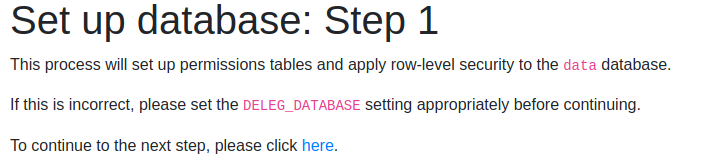
\includegraphics[scale=0.5]{02-setup1.png}
\end{center}

Following this, the next stage in the process fetches data on the database tables from the Django configuration. It then queries the database itself for information on relationship models (see implementation section for more details) and presents the user with a setup page to choose which tables and fields should be used when implementing the row-level security policies:

\begin{center}
  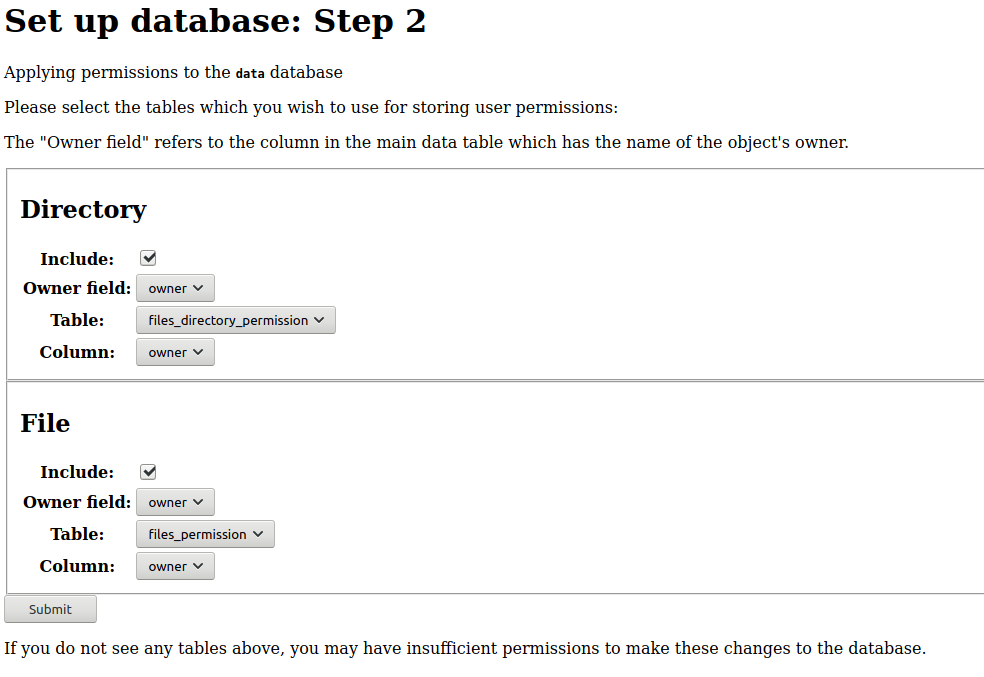
\includegraphics[width=\textwidth]{03-setup2.png}
\end{center}

Note the access control to this page is not critical (although it may be desirable to avoid confusing users). If an unauthorised user attempts to access this page, they will likely see no tables listed here (as the warning at the bottom of the previous image describes) due to not having access privileges to PostgreSQL's \verb+information_schema+ tables that hold metadata about the databases. Even if a user does have this access but is not authorised to create database policies, the following step will simply fail with a database permissions error. This is another illustration of the advantages of this approach over a traditional web application setup -- as long as the database access rights are set appropriately, the web app does not need extra security protection mechanisms.

Finally, a ``completion'' screen is shown. Following a successful operation this is blank, and error messages are reproduced here if the database engine returned an error:

\begin{center}
  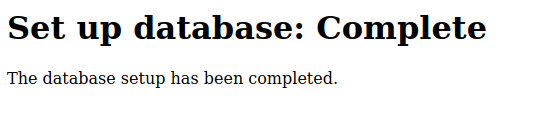
\includegraphics[scale=0.5]{04-setup3.png}
\end{center}

\subsection{Demonstration Application (File Browser)}
As a practical illustration of how the technology works, I developed a file browser application which allows a user to create, view and edit ``files'' (which, for demonstration purposes, are simple text entries stored in the database) and assign permissions to other users.

The basic interface shows a hierarchical directory structure with files and directories, and options to create new records:

\begin{center}
  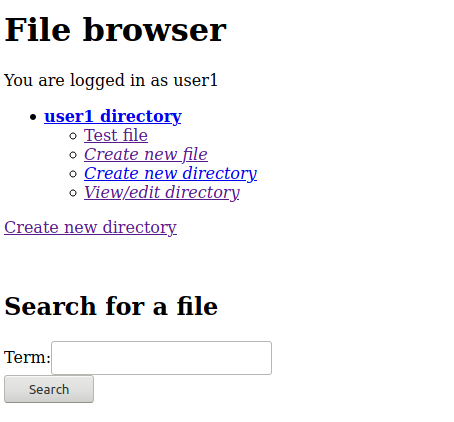
\includegraphics[scale=0.5]{05-browser1.png}
\end{center}

Each file and directory has a permissions interface visible to the registered ``owner'' of that record, to allow that user to add or remove permission entries:

\begin{center}
  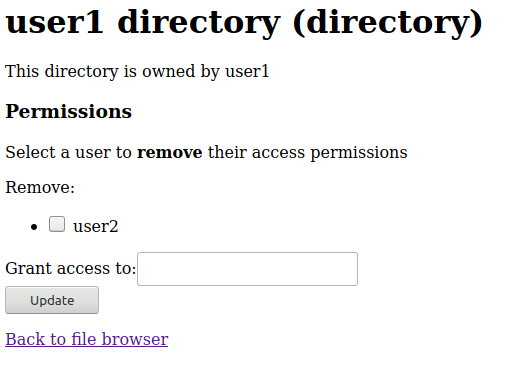
\includegraphics[scale=0.5]{06-browser2-perms.png}
\end{center}

In addition, file contents can easily be updated by the file owner (other users who have permission to access the file have read-only access -- this could easily be augmented to allow a more complex access control mechanism with separate read/write permissions that could be assigned to users):

\begin{center}
  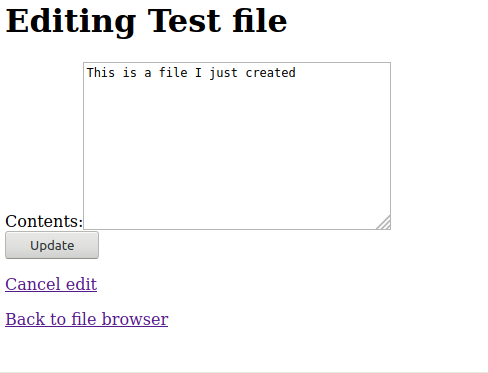
\includegraphics[scale=0.5]{07-browser3-file-contents.png}
\end{center}

The search feature of the app helps to demonstrate the security of the Kerberos delegation approach in that it contains a (deliberate) SQL injection vulnerability. The search function performs the following query (where \texttt{term} is a string provided by the user):

\begin{verbatim}
query = "SELECT * FROM " + table + "
         WHERE CONTENTS LIKE '%%" + term + "%%'"
\end{verbatim}

This can trivially be exploited by passing a search term such as \verb+' OR 1=1;--+ (as detailed in \autoref{sec:sql_injection}), and the web app's response shows that it is indeed vulnerable to SQL injection:

\begin{center}
  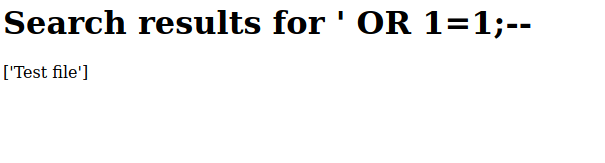
\includegraphics[scale=0.5]{08-browser4-sql.png}
\end{center}

However, this does not disclose any information which \texttt{user1} cannot access anyway. Note that counting all files in the database (running the count as the database super-user) shows that there are actually many more files than were extracted using the SQL injection:

\begin{verbatim}
filedb2=# SELECT owner, COUNT(*) AS TOTAL FROM files_file GROUP BY owner;
 owner  | total
--------+-------
 django |     6
 ***    |     2
 user1  |     1
(3 rows)
\end{verbatim}

(Note that the entry marked \verb+***+ was changed from the real command output to remove a personal identifier.)

This therefore demonstrates how \textbf{the presence of an SQL injection vulnerability in the constructed application does not allow unauthorised access to data}.

\section{Protocol Execution}
\label{sec:protocol_execution}
Using an approach without session cookies, a simple request to the webserver produces a sequence of packets such as the following:

\begin{center}
  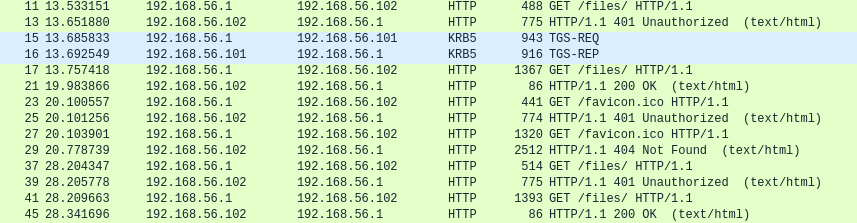
\includegraphics[width=\textwidth]{09-connect-no-cookie.png}
\end{center}

This sequence of packets shows an initial HTTP request from the client (192.168.56.1) to the web server (192.168.56.102), which sends back a response (HTTP 401) asking the user to authenticate. The client then requests and obtains a Kerberos service ticket from the Kerberos server (192.168.56.101), makes another request to the web server \textbf{with} this ticket, and receives the page contents as an HTTP response.

Each of the following requests in the sequence of packets repeats this cycle: although the client already has the service ticket, it must still make an initial HTTP request, receive a response requesting authentication and send another HTTP request with the service ticket. This is clearly inefficient, and so session cookies (as described in \autoref{sec:credential_cacheing}) are used in this application.

Once session cookies are enabled, the sequence of packets appears as follows:

\begin{center}
  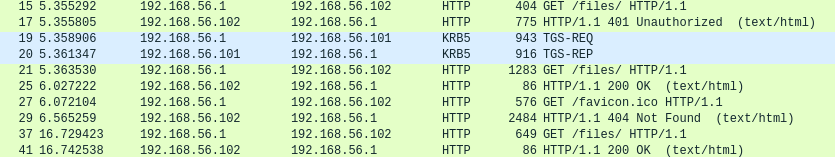
\includegraphics[width=\textwidth]{10-connect-cookie.png}
\end{center}

The initial exchange is effectively identical to the previous setup. However, the HTTP response in packet 25 now includes a session cookie, which is sent back by the browser in the subsequent requests. This means that the client can now request resources as ``standard'' HTTP requests (with no need to repeat the negotiation process), and so the efficiency of the system is increased (see \autoref{sec:performance_evaluation}).

See \autoref{sec:appendix4} for a protocol trace from the perspective of the client. This includes setting a session cookie, but the negotiation process illustrated is the same whether or not session cookies are used.


\begin{landscape}
  \section{Creation of Database Rules}
  The row-level security rules created by the database setup process can be inspected by directly logging in to the database server and using the PostgreSQL \verb+\dp+ command to list all privilege configurations on the current database. Doing this for the database after running the setup application produces the following result:

  (N.B. the ``Schema'' and ``Column privileges'' columns are included in the output from PostgreSQL, but do not show any useful information here and have been omitted from this document for space reasons. Some additional line breaks have also been added to the raw output to fit it into this document.)
  {\footnotesize
\begin{verbatim}
filedb2=# \dp
                                                    Access privileges
               Name                |   Type   |   Access privileges   |                         Policies
-----------------------------------+----------+-----------------------+-----------------------------------------------------------
 django_migrations                 | table    |                       |
 django_migrations_id_seq          | sequence | django=rwU/django    +|
                                   |          | =rU/django            |
 files_directory                   | table    | django=arwdDxt/django+| files_directory_view (r):                               +
                                   |          | =arw/django           |   (u): ( SELECT files_directory_permitted(
                                                                                 files_directory.id)
                                                                                 AS files_directory_permitted)                  +
                                   |          |                       | files_directory_view_owner:                             +
                                   |          |                       |   (u): ((owner)::text = SESSION_USER)                   +
                                   |          |                       | files_directory_insert (a):                             +
                                   |          |                       |   (c): true
 files_directory_id_seq            | sequence | django=rwU/django    +|
                                   |          | =rU/django            |
 files_directory_permission        | table    | django=arwdDxt/django+| files_directory_permission_owner:                       +
                                   |          | =ard/django           |   (u): (directory_id IN ( SELECT files_directory.id     +
                                   |          |                       |    FROM files_directory                                 +
                                   |          |                       |   WHERE ((files_directory.owner)::text = SESSION_USER)))+
                                   |          |                       | files_directory_permission_view (r):                    +
                                   |          |                       |   (u): ( SELECT files_directory_permitted(
                                                                                 files_directory_permission.directory_id)
                                                                                 AS files_directory_permitted)                  +
                                   |          |                       | files_directory_permission_insert (a):                  +
                                   |          |                       |   (c): (directory_id IN ( SELECT files_directory.id     +
                                   |          |                       |    FROM files_directory                                 +
                                   |          |                       |   WHERE ((files_directory.owner)::text = SESSION_USER)))
 files_directory_permission_id_seq | sequence | django=rwU/django    +|
                                   |          | =rU/django            |
 files_file                        | table    | django=arwdDxt/django+| files_file_view (r):                                    +
                                   |          | =arw/django           |   (u): ( SELECT files_file_permitted(files_file.id)
                                                                                 AS files_file_permitted)                       +
                                   |          |                       | files_file_view_owner:                                  +
                                   |          |                       |   (u): ((owner)::text = SESSION_USER)                   +
                                   |          |                       | files_file_insert (a):                                  +
                                   |          |                       |   (c): true
 files_file_id_seq                 | sequence | django=rwU/django    +|
                                   |          | =rU/django            |
 files_permission                  | table    | django=arwdDxt/django+| files_permission_owner:                                 +
                                   |          | =ard/django           |   (u): (file_id IN ( SELECT files_file.id               +
                                   |          |                       |    FROM files_file                                      +
                                   |          |                       |   WHERE ((files_file.owner)::text = SESSION_USER)))     +
                                   |          |                       | files_permission_view (r):                              +
                                   |          |                       |   (u): ( SELECT files_file_permitted(
                                                                                 files_permission.file_id)
                                                                                 AS files_file_permitted)                       +
                                   |          |                       | files_permission_insert (a):                            +
                                   |          |                       |   (c): (file_id IN ( SELECT files_file.id               +
                                   |          |                       |    FROM files_file                                      +
                                   |          |                       |   WHERE ((files_file.owner)::text = SESSION_USER)))
 files_permssion_id_seq            | sequence | django=rwU/django    +|
                                   |          | =rU/django            |
(10 rows)
\end{verbatim}
  }

  This demonstrates the correct operation of the setup procedure, with suitable constraints on viewing records based on ownership of information (and corresponding to the SQL queries made in the application code).

\end{landscape}

\section{Potential Attacks and Vulnerabilities}

\subsection{SQL Injection}
As demonstrated above, the presence of an SQL injection vulnerability (even one that allows arbitrary SQL execution) does not weaken the threat model of the system. The web app simply acts as a ``window'' onto the database to execute queries with the privileges of the user logged into the web app, and a user could just as easily use the same Kerberos ticket to log into the database server directly. This contrasts favourably with traditional systems where the web app itself is trusted to access the data of any user and so SQL injection vulnerabilities must be avoided.

\subsection{Theft of Long-Term Secrets}
As discussed in \autoref{sec:web_application_security}, the possible presence of passwords or other access tokens in source code can cause a risk of improper access if the secrets are not adequately protected. In many cases, database passwords such as these can be used from anywhere on the internet to gain access to all records in the database.

In this application, all authentication to the database is done using Kerberos tickets, and so there is no possibility of directly stealing a database key. However, it is important to note that the approach is still not entirely free of long-term secrets since they are still used in two significant contexts:
\begin{itemize}
\item
  Django's \verb+SECRET_KEY+ is stored in the Django filesystem and used for signing session cookies. Although this is certainly a potential security risk, in this case the Django session is only used for storage of database metadata between requests in the database setup application. Therefore, being able to break or forge these cookies would not provide a substantial advantage to an attacker since the PostgreSQL permissions setup would stop any genuine malicious activity on the database.
\item
  Apache's \verb+mod_session+ module is used to provide a session cookie that holds details of a user's authentication status. This represents a compromise to provide more usability at the expense of a slight loss in security, since if the signing key for these cookies were stolen an attacker would be able to impersonate any user who still had a cached ticket on the server. While this is still a clear improvement on a single master password (which if stolen could lead to \textbf{any} user being impersonated), it is nevertheless still a potential issue in some environments. It would easily be possible to dispense with this session cookie (if required) for security, but at the expense of a substantial performance reduction (see \autoref{sec:performance_evaluation}).

  This key is also substantially harder for an attacker to obtain since it is not stored anywhere in the directory structure of the web app itself and incorporates a randomly generated element which means that the key changes (at least) when the server is restarted. Therefore, in all likelihood, stealing this key is not a practical attack against the system.
\end{itemize}

\subsection{Data Obtainable from the Database}
One consequence of using delegated Kerberos tickets for accessing data is that users are given direct access to the database (which they potentially would not have had otherwise). This means that access control must be set up in the database itself, and this may offer a less granular permission model than could be specified if it were controlled by the web app (although the use of SQL stored procedures would allow a relatively broad set of options).

An example of a (minor) data leak caused by this setup is that it is possible to determine whether an object ID has already been allocated based on whether an \texttt{INSERT} operation with that ID succeeds or fails. On the assumption that these IDs are opaque identifiers such as sequential numbers (as they are in the example application), this is not significant, but if the ID contained useful information about the object then this would be a possible covert channel to leak information out.

\subsection{Theft of Credential Caches}
\label{sec:theft_of_credential_caches}
If a malicious user could execute a process on the web server (under the same system user account as the server application), that process would gain the same access to the credential cache directory that the web server application has.

Because of the patch added to \verb+mod_auth_gssapi+ and the directory permissions being set as described in \autoref{sec:credential_cacheing}, a malicious user could only enumerate files in the credential cache directory by doing a brute-force search on filenames. Given that each ticket is only useful for a small length of time, adding a suitably long random string to the filename should ensure that this method of obtaining tickets is not viable. To note further mitigations of the risks of credential caches being stolen:

\begin{itemize}
\item
  The tickets stored in these caches are service tickets, which can only be used on this web server and any services which it is allowed to delegate to. Unlike a password or a Kerberos ticket-granting ticket, they cannot be used on arbitrary other systems.
\item
  The only valid tickets that will be on the web server at all are those of users who have recently logged into it. Other users in the organisation will not have any ``live'' ticket data cached on the webserver, and so their data is not vulnerable even if the web server is compromised.
\end{itemize}

\subsection{Compromise of the Django Application}
A malicious user who is able to compromise the Django application itself would be able to see all data flowing through the compromised session, since the web app must have access to the data in order to display it.

The credential caches of users actively using the compromised application would also be available the attacker, subject to the same mitigation that these are server-restricted service tickets. As in \autoref{sec:theft_of_credential_caches}, a brute-force attack to obtain all credential caches on the system would be technically possible, but should be infeasible given the time taken. There is still no method of obtaining data on behalf of users who have not recently logged into the system.

\subsection{Compromise of the Whole Webserver}
Given a root-level compromise of the webserver, all cached credentials would be available to be stolen by an attacker since the root user can override file system access control policies. Any of these tickets could then be used to fetch data from the database, but note that two of the mitigating factors stated in \autoref{sec:theft_of_credential_caches} still apply: these are still service tickets which can only be used on a limited number of systems, and there is no effect on the security of users who have not recently logged into the web server.

\section{Performance Evaluation}
\label{sec:performance_evaluation}
A legitimate concern in building this project is the risk of degraded performance. Since the HTTP Negotiate protocol requires a multi-way ``handshake'' before starting data transfer, a na\"ive implementation of this project result in much slower access times than with a traditional web app.

Therefore, I measured the access times to reach the file browser main page (which involves requesting data from the database) in each of the following configurations:
\begin{itemize}
\item
  No database security at all (unlikely in reality, but serves as a baseline)
\item
  Database authentication with a master password (the typical real-world model)
\item
  Access via HTTP-Negotiate and delegated Kerberos tickets, using ticket cacheing on the web server and session cookies (as described in \autoref{sec:credential_cacheing}, and implemented in this project)
\item
  Access via HTTP-Negotiate and delegated Kerberos tickets, but \textbf{without} use of session cookies
\end{itemize}

Each of these access times was recorded 200 times in succession to allow summary statistics (median and quartiles) to be calculated. In addition, I measured the connection times (in both cases to a VM on my laptop running the web server) from my laptop and from a Microsoft Azure VM via an SSH tunnel to give some simulation of the effect of network latency.

\subsection*{Response Times (milliseconds)}
\begin{tabular}{|l|l|l|l|l|l|l|}
  \cline{3-7}
  \multicolumn{2}{l}{} \vline
  & \textbf{Min.} & \textbf{Quartile 1} & \textbf{Median} & \textbf{Quartile 3} & \textbf{Max.}\\
  \hline
  \multirow{4}{*}{\textbf{Laptop}}
  & No security & 21.1 & 23.4 & 24.8 & 26.4 & 57.0\\
  \cline{2-7}
  & Master password & 20.7 & 25.6 & 27.8 & 29.8 & 377\\
  \cline{2-7}
  & \makecell[l]{Kerberos with \\ session cookies} & 19.7 & 24.1 & 26.2 & 29.2 & 74.3\\
  \cline{2-7}
  & \makecell[l]{Kerberos without \\ session cookies} & 104 & 169 & 210 & 824 & 2070 \\
  \hline
  \multirow{4}{*}{\makecell[l]{\textbf{Azure} \\ \textbf{VM}}}
  & No security & 38.2 & 41.9 & 43.3 & 46.3 & 531\\
  \cline{2-7}
  & Master password & 38.7 & 41.7 & 42.7 & 44.3 & 459\\
  \cline{2-7}
  & \makecell[l]{Kerberos with \\ session cookies} & 38.2 & 40.5 & 41.5 & 43.2 & 111\\
  \cline{2-7}
  & \makecell[l]{Kerberos without \\ session cookies} & 125 & 183 & 209 & 838 & 2160\\
  \hline
\end{tabular}

Note that the ``Kerberos without session cookies'' data \textbf{excludes} the first connection of the session, where the cookie is obtained.

From the data above, there is a clear performance penalty from using HTTP negotiation without any form of session cookie, with the median access time rising from 20--45ms to over 200ms. There is also less significant, but noticeable, increase in access times when connecting from a remote location (particularly in the case of the maximum times, which would be expected given the possibility of packet loss or other connection issues).

To more easily visualise the data and analyse the performance of the system \textbf{with} session cookies enabled, I created box-plots (with outliers removed) of first three rows of data for each of the two connection sources:

\begin{center}
  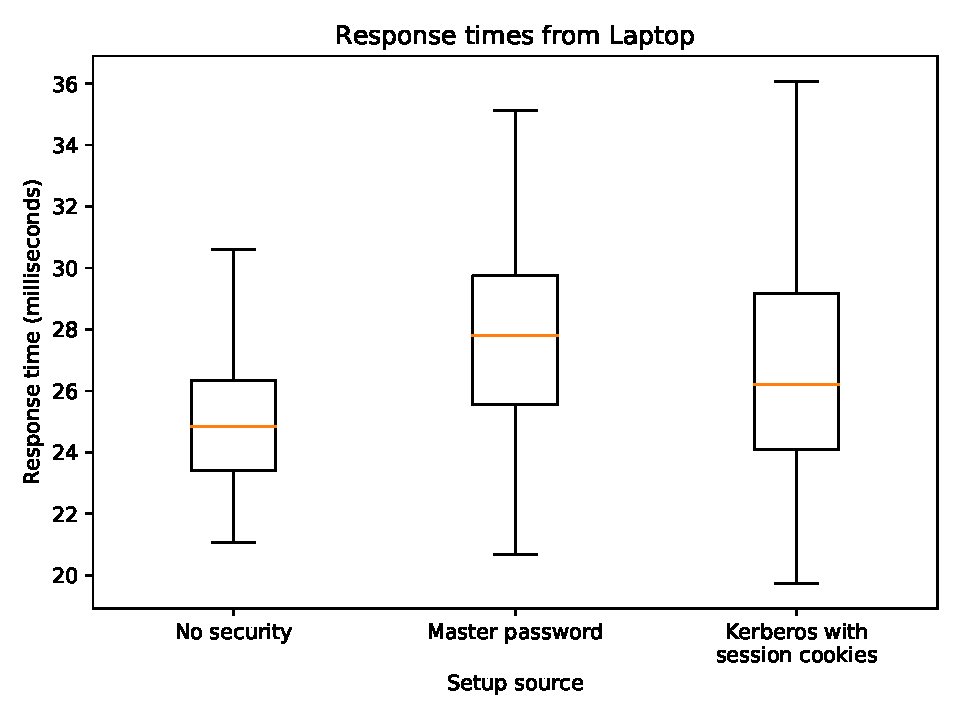
\includegraphics[width=0.8\textwidth]{11-response-times-laptop.pdf}
\end{center}

\begin{center}
  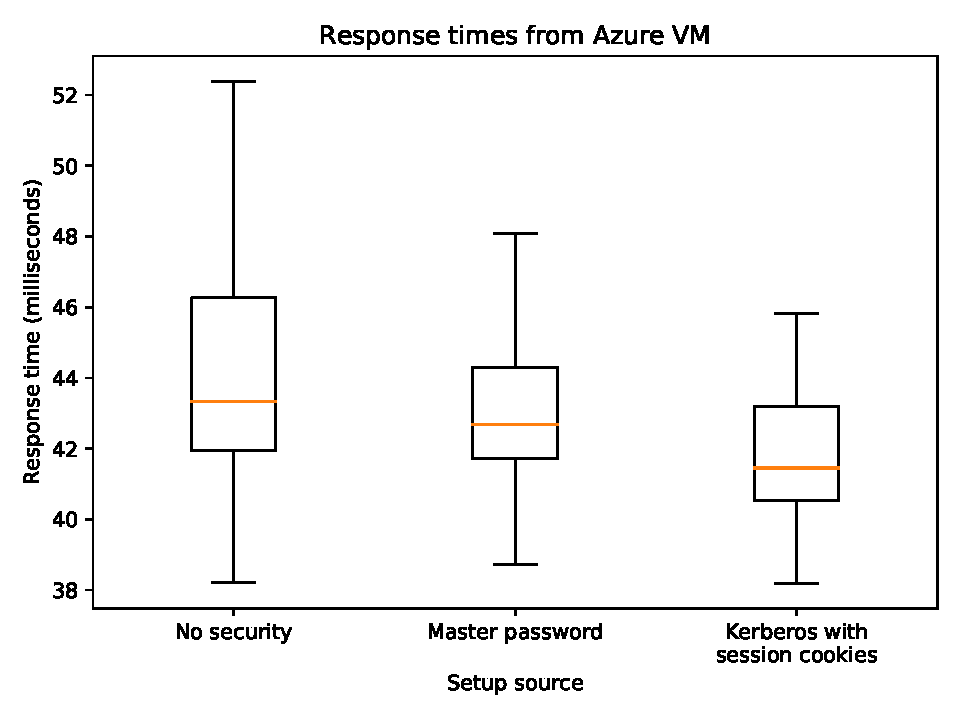
\includegraphics[width=0.8\textwidth]{12-response-times-azure.pdf}
\end{center}

From these plots, there is no indication of a reduction in performance compared with the use of a master database password (in fact the median values suggest a slight speed improvement, although the natural variation in the data means that the two approaches probably offer roughly equal performance in practice).

Although there is the overhead of the initial request to obtain the session cookie before the response times above are achievable, the same would apply to any single sign-on system (where a user is normally redirected to an external server for authentication, as in the OAuth2 protocol). Therefore, the performance overheads associated with this system should not be noticeably greater than in existing single sign-on systems.

\chapter{Conclusion}
\section{Summary of Work Completed}
As the main component of this project, I produced a Django web application which both provides an interface for setting up appropriate SQL permissions on a database (for use with delegated Kerberos tickets) and demonstrates a use of the setup with a file browser application. I also wrote two patches to existing software codebases (PostgreSQL and \verb+mod_auth_gssapi+) to add functionality where this would be useful for the project's application.

\section{Future Work}
Further research on methods of storing delegated tickets is an obvious potential extension to this project: for example, using kernel keyrings rather than a filesystem-based credential cache could offer a number of security advantages if the process-privacy issue can be resolved and the libraries (particularly \verb+mod_auth_gssapi+) suitably extended to work with it.

There is also clearly potential to use delegated Kerberos tickets for services beyond database servers. For example, extending the system to work with a network-based filestore using NFS would give a more flexible system than one which is specifically designed to access a database server, and introduce some nuances which are not covered by the scope of the current project (such as the fact that the OS kernel of the web server would likely need to be involved in the process of connecting to the NFS server).

\section{Lessons Learned}
As well as an exploration into the setup and use of Kerberos-based applications, this project also served as my first major experience of working on an existing open-source codebase. The time required to do this was fairly significant compared with the eventual volume of code written (in the form of the patches), and required preparatory work to understand the code structure and method calls in the hope of avoiding introducing any new bugs.

In some cases, I also began work on project components without a full enough understanding of the options available. For example, my initial implementation of the database security setup (using views and abstract classes), while functional, was inelegant and I would have used row-level security constructs from the start if I had developed a proper understanding of the options available at an earlier stage.

The process of developing the software, and discussions with my supervisor and the open-source project maintainers, was also a very useful learning experience, especially with regard to identifying potential security vulnerabilities in the system.


\begin{thebibliography}{99}
\bibitem{OWASP10} OWASP \textit{Top 10 Web Application Security Risks} list. \url{https://owasp.org/www-project-top-ten/} (accessed 21/10/2020)

\bibitem{GitGuardian} GitGuardian: Git Security Scanning \& Secrets Detection \url{https://www.gitguardian.com/} (accessed 22/04/2021)

\bibitem{GDPR} Data Protection Act 2018: Section 157 \url{https://www.legislation.gov.uk/ukpga/2018/12/section/157/enacted} (accessed 10/02/2021)

\bibitem{Oracle-OAuth2} Oracle OAuth Guide: API Gateway OAuth 2.0 Authentication Flows \url{https://docs.oracle.com/cd/E50612_01/doc.11122/oauth_guide/content/oauth_flows.html} (accessed 08/04/2021)

\bibitem{RFC2478} Eric Baize and Denis Pinkas (December 1998), \textit{The Simple and Protected GSS-API Negotiation Mechanism} (RFC 2478): \url{https://tools.ietf.org/html/rfc2478} (accessed 22/04/2021)

\bibitem{RFC2743} John Linn (January 2000), \textit{Generic Security Service Application Program Interface Version 2, Update 1} (RFC 2743): \url{https://tools.ietf.org/html/rfc2743} (accessed 26/04/2021)

\bibitem{RFC2744} John Wray (January 2000), \textit{Generic Security Service API Version 2 : C-bindings} (RFC 2744): \url{https://tools.ietf.org/html/rfc2744.html} (accessed 26/04/2021)

\bibitem{RFC4178} Larry Zhu et.\ al.\ (October 2005), \textit{The Simple and Protected Generic Security Service Application Program Interface (GSS-API) Negotiation Mechanism} (RFC 4178): \url{https://tools.ietf.org/html/rfc4178} (accessed 26/04/2021)

\bibitem{RFC4559} Karthik Jaganathan, Larry Zhu and John Brezak (June 2006), \textit{SPNEGO-based Kerberos and NTLM HTTP Authentication in Microsoft Windows} (RFC 4559): \url{https://tools.ietf.org/html/rfc4559} (accessed 04/04/2021)

\bibitem{KDC-database-docs} MIT Kerberos documentation: Database Types \url{https://web.mit.edu/kerberos/krb5-devel/doc/admin/conf_ldap.html} (accessed 05/05/2021)

\bibitem{KRB-DELEG} Kerberos: delegation and s4u2proxy (Simo Sorce, 12/02/2012) \url{https://ssimo.org/blog/id_011.html} (accessed 02/02/2021)

\bibitem{JohnKol-unconstrained-deleg} Ioannis Kollitidis (March 2020), Unconstrained Delegation: \url{https://johnkol.com/unconstrained-delegation/} (accessed 27/04/2021)

\bibitem{KDC-conf-docs} MIT Kerberos documentation: \texttt{kdc.conf} \url{https://web.mit.edu/kerberos/www/krb5-devel/doc/admin/conf_files/kdc_conf.html} (accessed 05/04/2021)

\bibitem{MS-s4u2} Microsoft Corporation (May 2014), \textit{Kerberos Protocol Extensions: Service for User and Constrained Delegation Protocol}: \url{https://winprotocoldoc.blob.core.windows.net/productionwindowsarchives/MS-SFU/[MS-SFU]-140515.pdf} (accessed 05/04/2021)

\bibitem{MS-deleg-attribute} Microsoft Corporation (February 2019), Attribute \texttt{msDS-AllowedToDelegateTo} \url{https://docs.microsoft.com/en-us/openspecs/windows_protocols/ms-ada2/86261ca1-154c-41fb-8e5f-c6446e77daaa} (accessed 05/05/2021)

\bibitem{MIT-ccache-types} MIT Kerberos documentation: Credential cache \url{https://web.mit.edu/kerberos/krb5-devel/doc/basic/ccache_def.html} (accessed 25/04/2021)

\bibitem{postgres-SEC_DEF} PostgreSQL documentation: \texttt{CREATE FUNCTION} \url{https://www.postgresql.org/docs/current/sql-createfunction.html#SQL-CREATEFUNCTION-SECURITY} (accessed 22/02/2021)

\bibitem{postgres-CREATE_VIEW} PostgreSQL documentation: \texttt{CREATE VIEW} \url{https://www.postgresql.org/docs/13/sql-createview.html} (accessed 05/05/2021)

\bibitem{postgres-CREATE_RULE} PostgreSQL documentation: \texttt{CREATE RULE} \url{https://www.postgresql.org/docs/current/sql-createrule.html} (accessed 22/02/2021)

\bibitem{Apache-book} Kew, Nick. (2007). The Apache modules book : Application development with Apache (1st ed., Prentice Hall open source software development series)

\bibitem{Django-docs} Django documentation (including the sub-pages linked from here) \url{https://docs.djangoproject.com/en/3.1/} (accessed 27/04/2021)

\bibitem{RFC4648} Simon Josefsson (October 2006), \textit{The Base16, Base32, and Base64 Data Encodings} (RFC 4648): \url{https://tools.ietf.org/html/rfc4648} (accessed 30/04/2021)

\bibitem{Apache-base64-commit} minifrin (June 2018), Revision 1834371 to Apache web server codebase: \url{https://svn.apache.org/viewvc?view=revision&revision=1834371} (accessed 30/04/2021)

\bibitem{postgres-policy} PostgreSQL documentation: \texttt{CREATE POLICY} \url{https://www.postgresql.org/docs/13/sql-createpolicy.html} (accessed 23/04/2021)

\bibitem{postgres-GSSAPI} PostgreSQL documentation: GSSAPI Authentication \url{https://www.postgresql.org/docs/13/gssapi-auth.html} (accessed 19/04/2021)

\bibitem{postgres-patch-list} \texttt{pgsql-hackers} mailing list, \textit{PATCH: Add GSSAPI ccache\_name option to libpq} \url{https://www.postgresql.org/message-id/flat/183cb0c3-30a9-149e-5403-fd36800e8c2b%40gmail.com} (accessed 06/05/2021) [N.B. link contains a personal identifier]

\bibitem{AcceptPathInfo-source} Apache web server source code: \texttt{AcceptPathInfo} \url{https://github.com/apache/httpd/blob/587d17015167f442c98efaf497504fe3825a3fe7/server/core.c#L3394} (accessed 02/05/2021)


\end{thebibliography}

\appendix
\chapter{Apache Configuration}
\label{sec:appendix1}
The following is the complete \verb+.htaccess+ file used to configure options in the Apache web server. This primarily demonstrates the setup of the \verb+mod_auth_gssapi+ module, including the new \texttt{Secure} mode for the \texttt{GssapiDelegCcacheUnique} parameter that was added as part of this project.

\begin{verbatim}
# Enable GSSAPI authentication
AuthType GSSAPI
AuthName "Kerberos site authentication"

# Only allow Kerberos authentication (not NTLM etc.)
GssapiAllowedMech krb5

# Enable delegation support
GssapiUseS4U2Proxy On

# Specify where keytab file for server principal is located
GssapiCredStore keytab:/var/www/apache.keytab
GssapiCredStore client_keytab:/var/www/apache.keytab

# Save delegated tickets to directory, and add random suffix to make
# them harder to brute-force
GssapiDelegCcacheDir /var/run/apache2/clientcaches
GssapiDelegCcacheUnique Secure

# Strip realm off user name (after Kerberos library has verified it)
GssapiLocalName On

# Use a session cookie to avoid having to negotiate on each request
GssapiUseSessions On
Session On
SessionCookieName session path=/;httponly;samesite=strict

# Only allow authenticated users to access the application
Require valid-user
\end{verbatim}

\chapter{Django Database Router}
\label{sec:appendix2}
The code below shows the routing process for Django to determine which database to use for a given type of request:

\begin{verbatim}
class FileDBRouter:
    APP_LABEL = 'files'

    DATA_DB = settings.DELEG_DATABASE
    DEFAULT_DB = 'default'

    def db_for_read(self, model, **hints):
        """
        File access goes to 'data' database, otherwise default
        """
        if model._meta.app_label == self.APP_LABEL:
            return self.DATA_DB
        return self.DEFAULT_DB

    def db_for_write(self, model, **hints):
        """
        File access goes to 'data' database, otherwise default
        """
        if model._meta.app_label == self.APP_LABEL:
            return self.DATA_DB
        return self.DEFAULT_DB

    def allow_relation(self, obj1, obj2, **hints):
        """
        Only allow relations within a database, not across multiple
        databases
        """
        return ((obj1._meta.app_label == self.APP_LABEL) ==
                (obj2._meta.app_label == self.APP_LABEL))

    def allow_migrate(self, db, app_label, model_name=None, **hints):
        """
        Only put files into the 'data' database, and everything else
        into the 'default' database
        """
        return (app_label == self.APP_LABEL) == (db == self.DATA_DB)
\end{verbatim}

The main database (\verb+DATA_DB+, whose name is stored in the general Django settings file as it is also required in the database setup procedure) contains the data to be protected by PostgreSQL access control. The ``default'' database (\verb+DEFAULT_DB+) is used for all other records (primarily web app session information), and so this router directs queries from the file browser app to the PostgreSQL database, and other data which is internal to the web app to the other database.

Once this router is in place, the routing is transparent to the web app, which simply needs to use the Django models classes as normal. The router can be overridden in an application if necessary, and this is done on the \verb+managedb+ pages to allow setup of the database permissions.

(The code above is loosely based on several examples given in the Django documentation at \url{https://docs.djangoproject.com/en/3.1/topics/db/multi-db/}.)

\chapter{\texttt{mod\_auth\_gssapi} Patch}
\label{sec:appendix3}

The following \texttt{diff} extracts (slightly altered for line length in this report) show more detail on the changes made to the \verb+mod_auth_gssapi+ module.

Calling of the subroutine to create a random string:

\begin{verbatim}
-    ccname = apr_psprintf(pool, "%s/%s-XXXXXX", dir, escaped);
+    if (use_random) {
+        const char *rand_string = get_random_string(16, req->pool);
+        ccname = apr_psprintf(pool, "%s/%s-%s-XXXXXX", dir, escaped,
+                              rand_string);
+    } else {
+        ccname = apr_psprintf(pool, "%s/%s-XXXXXX", dir, escaped);
+    }
\end{verbatim}

Implementing a multiple-choice option (rather than a simple on/off) flag:

(Based on the style used elsewhere in Apache code, for example in the \texttt{AcceptPathInfo} option\cite{AcceptPathInfo-source})

\begin{verbatim}
 static const char *mag_deleg_ccache_unique(cmd_parms *parms,
                                            void *mconfig,
-                                           int on)
+                                           const char *arg)
 {
     struct mag_config *cfg = (struct mag_config *)mconfig;
-    cfg->deleg_ccache_unique = on ? true : false;
+
+    if (ap_cstr_casecmp(arg, "on") == 0) {
+        cfg->deleg_ccache_unique = true;
+        cfg->deleg_ccache_random = false;
+    }
+    else if (ap_cstr_casecmp(arg, "off") == 0) {
+        cfg->deleg_ccache_unique = false;
+        cfg->deleg_ccache_random = false;
+    }
+    else if (ap_cstr_casecmp(arg, "secure") == 0) {
+        cfg->deleg_ccache_unique = true;
+        cfg->deleg_ccache_random = true;
+    }
+    else {
+        return
+        "GssapiDelegCcacheUnique must be set to on, off or secure";
+    }
     return NULL;
 }
\end{verbatim}

\chapter{HTTP Negotiate Protocol Trace}
\label{sec:appendix4}

\begin{verbatim}
$ curl -v --negotiate -u : krbsite.local/files/
*   Trying 192.168.56.102...
* TCP_NODELAY set
* Connected to krbsite.local (192.168.56.102) port 80 (#0)
> GET /files/ HTTP/1.1
> Host: krbsite.local
> User-Agent: curl/7.58.0
> Accept: */*
>
< HTTP/1.1 401 Unauthorized
< Date: Thu, 29 Apr 2021 16:21:40 GMT
< Server: Apache/2.4.41 (Ubuntu)
< WWW-Authenticate: Negotiate
< Content-Length: 460
< Content-Type: text/html; charset=iso-8859-1
<
* Ignoring the response-body
* Connection #0 to host krbsite.local left intact
* Issue another request to this URL: 'http://krbsite.local/files/'
* Found bundle for host krbsite.local: 0x56331d9c8ad0 [can pipeline]
* Re-using existing connection! (#0) with host krbsite.local
* Connected to krbsite.local (192.168.56.102) port 80 (#0)
* Server auth using Negotiate with user ''
> GET /files/ HTTP/1.1
> Host: krbsite.local
> Authorization: Negotiate YIICewYGKwYBBQUCoIICbzCCAmugDTALBgkqhkiG9...
> User-Agent: curl/7.58.0
> Accept: */*
>
< HTTP/1.1 200 OK
< Date: Thu, 29 Apr 2021 16:21:40 GMT
< Server: Apache/2.4.41 (Ubuntu)
< WWW-Authenticate: Negotiate oYG3MIG0oAMKAQChCwYJKoZIhvcSAQICooGfBIG...
< Set-Cookie: session=MagBearerToken=fGZU6v8uKhalBbmvCLOYfeHsN5JLLTg3...;
  path=/;httponly;samesite=strict
< Cache-Control: no-cache, private
< Content-Length: 2031
< X-Frame-Options: DENY
< X-Content-Type-Options: nosniff
< Referrer-Policy: same-origin
< Vary: Accept-Encoding
< Content-Type: text/html; charset=utf-8
\end{verbatim}
[The page content now follows]

\chapter{Project Proposal}
\title {{\Large Computer Science Tripos -- Part II -- Project Proposal}\\ \vspace{10mm} Kerberos-based single sign-on with delegation for web applications}

\author {Candidate 2428G \\ Originator: Dr Markus Kuhn}

\date {October 22, 2020}

\documentclass{article}
\usepackage[margin=1in, a4paper]{geometry}
\usepackage{parskip}
\usepackage[pdfauthor={Candidate 2428G}, pdftitle={Project Proposal}, pdfsubject={Kerberos-based single sign-on with delegation for web applications}]{hyperref}
%\usepackage{cprotect}

\begin{document}
\maketitle

\textbf{Project Supervisor}: Dr Markus Kuhn

\textbf{Director of Studies}: Dr Robert Harle

\textbf{Overseers}: Professor Frank Stajano and Dr Amanda Prorok


\section*{Project Description}
Many web applications are built around databases, and traditionally the application itself has full access to any database records and controls access to them by users. This means that security vulnerabilities in the application or framework can result in incorrect access or modification to data, with potentially severe consequences -- a simple vulnerability in a custom-written web application could allow an attacker to access other site users’ personal data.

Kerberos authentication works on the basis of each user getting a ``ticket'' which can be used to gain access to other systems, and so this project aims to set up a system where users can authenticate to a web application via Kerberos, and where there is no ``global secret'' that allows the web application to access all database records. Therefore, as long as the database access rights are set correctly, there is no need for the front-end to perform access control.

The project will involve adding to the Django framework (in the form of a plugin) so that it can receive authenticate a user via a Kerberos ticket, pass that ticket on to a database, and then access that user’s data from the database. Basic Kerberos authentication functionality already exists in Django modules, but this is only designed for authenticating to the web app itself and not passing a Kerberos ticket onto the database.

This will mean that a user can obtain a Kerberos ticket, then use that to authenticate to the website (using the HTTP Negotiate authentication scheme). The same ticket could be used for multiple different sites that are set up in this way, and so it effectively forms a single sign-on system. The web server itself should not have access to database records except via the Kerberos tickets.

To the user, this will mean that they can provide a Kerberos ticket to any site which is part of this system (and is in the same Kerberos ``realm''). Quite apart from the standard benefits of a single sign-on system (only one password required for a whole set of sites, which means that users are more likely to be able to remember a strong password and less likely to record it using insecure methods), this would mean that SQL injection (a type of command injection, which is currently number 1 in the OWASP \textit{Top 10 Web Application Security Risks} list) would not result in any data being disclosed beyond what a user had access to anyway. This is because the database itself would be implementing the security restrictions, and eliminates a significant vulnerability faced by many web applications.

An important aspect of the project is how Kerberos tickets are stored on the web server. Existing technologies often simply store all tickets in a directory on the server, and this makes them vulnerable to any other site running on the same system being able to read and use the tickets. By investigating and building a better means for storing tickets, a compromised site should not mean that all other web sites on the server are automatically also compromised.

\section*{Starting Point}
Kerberos support for Apache already exists (via the \verb+mod_auth_gssapi+ module and the older \verb+mod_auth_kerb+ module), and this includes some ability to delegate tickets although with drawbacks (particularly that tickets to be delegated are placed in a directory which is accessible to any process running as the webserver user). Django similarly includes Kerberos extensions (such as \verb+django-gssapi+), but these do not directly offer any delegation facilities. As a starting point, I will investigate these and build on the functionality which they already offer.

PostgreSQL already has support for Kerberos and this can be used as a back-end database system.

I have some knowledge of authentication systems and general security topics from the 1B Security course, and of C programming from the 1B Programming in C and C++ course. I have also had general experience with web application setup (although not the specific technologies involved here) through the 1B Group Project and work done outside the Tripos.

In addition, over the summer vacation I have done some experimentation with Kerberos authentication to set up a virtual machine using the existing Kerberos functionality of Apache and PostgreSQL (logging in separately to the two applications without any delegation of tickets).

\section*{Work to be done}
\begin{enumerate}
\item Familiarity with the structure of Kerberos authentication (and MIT Kerberos specifically)
\item Familiarity with Apache web server development (as modifications to the Apache modules may be necessary)
\item Setting up a environment with a suitable web application and Kerberos server
\item Implementation and testing of the authentication functionality
\item Modularising the setup to work as a Django module
\item Evaluation of the performance and security of the system
\end{enumerate}

\section*{Success Criteria}
\begin{itemize}
\item The project will consist of an add-on to the Django framework which offers Kerberos authentication.
\item A user must be able to log into the web application by presenting a suitable Kerberos ticket, which the application then uses to fetch data from a database.
\item The application must not have access to the database other than by Kerberos tickets (so a given piece of data cannot be fetched without a Kerberos ticket corresponding to a principal who has access to that data). This means that a given user cannot access data which they are not authorised to have access to, even in the presence of web app vulnerabilities.
\end{itemize}

\section*{Evaluation}
In order to evaluate the functionality, I will develop a basic web application which allows a user to manage an access control list associated with a resource they have uploaded, so as to permit or deny other users access to it. The aim of the project is to enforce this access policy on the SQL server, so that even in the presence of a vulnerability in the web app front-end where arbitrary SQL code could be executed by a user, the access control policy would not be broken.

As a result of this, it is important that the SQL server always ``agrees'' with the web app on who is accessing a page. If this can be demonstrated to be the case, then security vulnerabilities in the web app would not allow and inappropriate access to data, because the authorisation (and authentication) steps would all be performed by the database system.

Uses for this system could include web-based file systems (where a user can upload files and grant certain other users permission to see it), with each user registered as a separate ``user'' in the SQL database. The web app itself would not perform any security and would merely act as a front-end to pass the user's Kerberos ticket onto the database, where authentication and authorisation would occur.

Therefore, the evaluation will take the form of a security analysis of the system and how vulnerable it is to attacks, in particular via SQL injection (as well as also potentially looking at the effect if another site running on the same web server is compromised). In addition, I will measure the performance of the system to consider impacts on response times compared with a basic (non-Kerberos enabled) web app and database.

\section*{Timetable}
\subsection*{Michaelmas Weeks 4 to 5 (29/10 to 11/11)}
Set up a basic test environment for this project, with a web server and SQL database which can be queried by the site. At this stage, neither the web site itself nor its connection to the database would have any security.

Milestone: a test web application connecting to a database (without security)

\subsection*{Michaelmas Weeks 6 to 7 (12/11 to 25/11)}
Investigate existing Kerberos authentication libraries, and use them to set up authentication to the site (so that the site can access the user's Kerberos principal name, for example, and pull this user's data from a database). This would be done with a connection to a ``test'' Kerberos KDC (running locally in a VM). If possible, this will include using existing ticket delegation functionality in Apache.

Milestone: authentication to the web application itself via Kerberos (using existing technologies)

\subsection*{Michaelmas Week 8 to Vacation Week 3 (26/11 to 23/12)}
Work on adding and improving the ticket delegation functions of the system, so that a user to this (particular) application can supply a Kerberos ticket which is used to access database resources. This includes evaluating approaches to storing tickets, ensuring that the delegation process works properly, and fixing any issues that arise.

Milestone: able to log into a single web application and delegate the Kerberos ticket to a database

\subsection*{Vacation Weeks 4 to 7 (24/12 to 20/01)}
Modularise the previously built delegation code, so that it can be used as a plug-in with any suitable site based on the Django framework. Test use of this plug-in and fix any further issues.

Milestone: Kerberos ticket delegation system as a web framework plug-in

\subsection*{Lent Weeks 1 to 2 (21/01 to 03/02)}
Contingency time to fix any remaining issues and further test the system.
Write mid-project report, and (if possible) begin writing up the project.

Milestone: project report

\subsection*{Lent Weeks 3 to 4 (04/02 to 17/02)}
Continue to write up the project.

Look into possible improvements to further reduce the vulnerability of the system.

\subsection*{Lent Weeks 5 to 6 (18/02 to 03/03)}
Finish draft write-up (continue working on extensions if ahead of schedule). Submit to supervisor for review.

Milestone: draft dissertation

\subsection*{Lent Weeks 7 to 8 (04/03 to 17/03)}
Time for supervisor to read and comment on report.

Work on extensions if time permits (N.B. reduced time available due to Unit of Assessment).

\subsection*{Vacation Weeks 1 to 6 (18/03 to 28/04)}
Modifications and changes to the report based on feedback.

Complete full write-up, aiming to be ready to submit at the start of Easter term. If further time is available, then continue to work on extensions.

Milestone: dissertation complete

\subsection*{Easter Weeks 1 to 2 (29/04 to 12/05)}
Contingency time to deal with any last-minute issues and problems.

Deadline: Friday 14th May 2021

\section*{Resources required}
I plan to use my own computer (quad-core 1.6GHz CPU, 12GB RAM, 1TB hard drive, Linux Mint OS).

Source code will be held in a GitHub repository, with a copy uploaded to Dropbox each day and weekly backups made to an external hard drive.

This means that, in the event of hardware or software failure, I will be able to transition work to a replacement machine or to the MCS. I accept full responsibility for this machine and I have made contingency plans to protect myself against hardware and/or software failure.

\section*{Possible extensions}
\begin{itemize}
\item Investigate using the same SQL server to record web server logs -- this would require the web server application to switch Kerberos tickets between the client's ticket (to access client resources) and its own ticket (which would have access to server log tables), and ensure that this process of switching did not impact on the security of the system.
\item Investigate whether this could be extended to access files over NFS via the same process of ticket delegation from a web application.
\end{itemize}

\section*{Bibliography}
\begin{itemize}
\item \url{https://www.cl.cam.ac.uk/~mgk25/project-ideas/#http-gssapi} (accessed 19/10/2020) \\ The project suggestion which this proposal is based on
\item \url{https://tools.ietf.org/html/rfc4178} (accessed 19/10/2020) \\ RFC 4178 (The Simple and Protected GSS-API Negotiation Mechanism), which describes the overall standard for Kerberos authentication to web applications
\item \url{https://tools.ietf.org/html/rfc4559} (accessed 19/10/2020) \\ RFC 4559 (SPNEGO-based Kerberos and NTLM HTTP Authentication in Microsoft Windows), describing a Microsoft-based system which offers similar functionality
\item \url{https://developer.mozilla.org/en-US/docs/Mozilla/Integrated_authentication} (accessed 19/10/2020) \\ Mozilla Integrated authentication documentation (a useful overall description of web application Kerberos authentication)
\item \url{https://github.com/gssapi/mod_auth_gssapi} (accessed 19/10/2020) \\ \verb+mod_auth_gssapi+ Apache module documentation
\item \url{https://pypi.org/project/django-gssapi/} (accessed 19/10/2020)  \\ \verb+django-gssapi+ documentation
\item \url{https://www.postgresql.org/docs/12/gssapi-auth.html} (accessed 19/10/2020) \\ Using PostgreSQL with GSSAPI
\item \url{https://web.mit.edu/kerberos/krb5-1.12/doc/} (accessed 19/10/2020) \\ MIT Kerberos documentation
\item \url{https://owasp.org/www-project-top-ten/} (accessed 21/10/2020) \\  OWASP \textit{Top 10 Web Application Security Risks} list
\end{itemize}

\end{document}

\end{document}
